%%%%%%%%%%%%%%%%%%%%%%%%%%%%%%%%%%%%%%%%%
% a0poster Portrait Poster
% LaTeX Template
% Version 1.0 (22/06/13)
%%%%%%%%%%%%%%%%%%%%%%%%%%%%%%%%%%%%%%%%%
% a0poster Portrait Poster
% LaTeX Template
% Version 1.0 (22/06/13)
%
% The a0poster class was created by:
% Gerlinde Kettl and Matthias Weiser (tex@kettl.de)
% 
% This template has been downloaded from:
% http://www.LaTeXTemplates.com
%
% License:
% CC BY-NC-SA 3.0 (http://creativecommons.org/licenses/by-nc-sa/3.0/)
%
%%%%%%%%%%%%%%%%%%%%%%%%%%%%%%%%%%%%%%%%%

%----------------------------------------------------------------------------------------
%	PACKAGES AND OTHER DOCUMENT CONFIGURATIONS
%----------------------------------------------------------------------------------------

\documentclass[20pt,a0,portrait]{a0poster}

\usepackage{multicol} % This is so we can have multiple columns of text side-by-side
\columnsep=100pt % This is the amount of white space between the columns in the poster
\columnseprule=3pt % This is the thickness of the black line between the columns in the poster
\usepackage[svgnames]{xcolor} % Specify colors by their 'svgnames', for a full list of all colors available see here: http://www.latextemplates.com/svgnames-colors

% \usepackage{times} % Use the times font
% \usepackage{palatino} % Uncomment to use the Palatino font


\usepackage{graphicx} % Required for including images
\graphicspath{{figures/}} % Location of the graphics files
\usepackage{booktabs} % Top and bottom rules for table
\usepackage[font=small,labelfont=bf]{caption} % Required for specifying captions to tables and figures
\usepackage{amsfonts, amsmath, amsthm, amssymb} % For math fonts, symbols and environments
\usepackage{wrapfig} % Allows wrapping text around tables and figures


%%%%%%%%%%%%%%%%%%%%%%%%%%%%%%%%%%%%%5

%Настройка русского языка
\usepackage[utf8]{inputenc}
\usepackage[T2A]{fontenc}
\usepackage[english, russian]{babel}
\selectlanguage{russian}

%\usepackage{anyfontsize}

%\usepackage{cite} % Работа с библиографией
%\usepackage[superscript]{cite} % Ссылки в верхних индексах
%\usepackage[nocompress]{cite} % 
%\usepackage{csquotes} % Еще инструменты для ссылок


\usepackage{caption}
\usepackage{subcaption}

\usepackage{palatino} 

\usepackage{floatrow} %for floating subscribes

\usepackage{anyfontsize} %Пакет для сзданя шрифтк крупного размера
\usepackage[noae]{Sweave}


\definecolor{coolblack}{rgb}{0.0, 0.18, 0.39}
\definecolor{darkblue}{rgb}{0.0, 0.0, 0.55}

%%%%%%%%%%%%%%%%%%%%%%%%%%%% Меняем парамтеры плавающих объектов
\usepackage{float}
\floatstyle{plaintop}
\restylefloat{table}


%%%%%%%%%%%%%%%%%%%%%%%%%%%%%%%%%%%%%

\usepackage{fancyref}

\usepackage{natbib} %Пакет для более человеческой библиографии
\usepackage{tempora}% for text если компиляция идет PDFLatex, то этот пакет активирует Times подобный шрифт.


% \usepackage{eso-pic,graphicx}
\usepackage[top=4cm, bottom=2cm, outer=1cm, inner=4cm]{geometry}


\begin{document}
\Sconcordance{concordance:Poster_MBS_2020_var2.tex:Poster_MBS_2020_var2.Rnw:%
1 283 1 1 118 55 1 1 96 96 1}


	%----------------------------------------------------------------------------------------
	%	POSTER HEADER 
	%----------------------------------------------------------------------------------------
	
	% The header is divided into two boxes:
	% The first is 75% wide and houses the title, subtitle, names, university/organization and contact information
	% The second is 25% wide and houses a logo for your university/organization or a photo of you
	% The widths of these boxes can be easily edited to accommodate your content as you see fit
	
	% \AddToShipoutPictureBG*{
\includegraphics[width=\paperwidth,height=\paperheight]{background}};
% \clearpage
	
	
	\begin{minipage}[b]{0.95\linewidth}
	\center
	
		\veryHuge \color{NavyBlue} \textbf{Star Wars and Angry Birds:}\\ 
		\Huge \color{NavyBlue} \textbf{морские звезды и кулики-сороки регулируют структуру смешанных поселений \emph{Mytilus edulis} и \emph{M.trossulus} в Белом море } \color{NavyBlue}\\ % Title
%		\veryHuge \textit{}\\[1cm] % Subtitle
	\end{minipage}

\vspace{1cm}
	\begin{minipage}[b]{0.75\linewidth}
		\Large \textbf{Вадим Хайтов,  Рената Нематова, Алена Евдокимова}\\[0.5cm] % Author(s)
		\large Лаборатория экологии морского бентоса (гидробиологи)\\[0.4cm] % University/organization
		\large Кандалакшский государственный заповедник\\[0.4cm] % University/organization
		\large Санкт-Петербургский государственный университет\\[0.4cm] % University/organization
		\large \texttt{polydora@rambler.ru}\\
	\end{minipage}
	%
	\begin{minipage}[b]{0.25\linewidth}
		
\includegraphics[width=15 cm]{logos.jpg}\\
	\end{minipage}
	
	\vspace{1 cm} % A bit of extra whitespace between the header and poster content
	
	%----------------------------------------------------------------------------------------
	
	%\begin{multicols}{2} % This is how many columns your poster will be broken into, a portrait poster is generally split into 2 columns
		
		%----------------------------------------------------------------------------------------
		%	ABSTRACT
		%----------------------------------------------------------------------------------------
		
		\color{Navy} % Navy color for the abstract
		
		
% Важно!!! У минипейджа должен стоять ключ [t] чтобы два минипейджа встали бок о бок

\begin{minipage}[t]{0.5\linewidth}		
		
% 		\begin{abstract}
% 			
% Мы показали, что  одним из факторов, регулирующих соотношение обилй \textit{M. edulis} и \textit{M. trossulus} в Белом море, могут являться хщники: морские звезды \textit{A. rubens} и кулки-сороки \textit{H. ostralegus}. Оба вида хищников сокращают относительное обилие \textit{M. trossulus} в смешанных поселениях.   
% 			
% 		\end{abstract}
% 		




		\color{Black} % SaddleBrown color for the introduction



\section*{\centering {Введение}}




%%%%%% Внимание! чтобы минипейджи ставились бок о бок надо между ними поставить знак "%"
		
%
\begin{minipage}[t][10cm][t]{0.4\textwidth}

Помимо коренного для Белого моря вида мидий (\emph{M.edulis}) во многих участках  Кандалакшского залива представлен инвазивный вид, \emph{M.trossulus}, который был занесенной в акваторию не более 80 лет назад. Высокая концентрация \emph{M.trossulus} наблюдается в кутовой части Кандалакшского залива (рис. \ref {Fig_distred}). Факторы, сдерживающие распространение  вида-вселенца, изучены слабо, но можно предположить, что некоторую роль в этом играют хищные животные, для которых мидии являются основным видом корма. К числу таких хищников относятся морские звезды (\emph{Asterias rubens}) и кулики-сороки (\emph{Haematopus  ostralegus}). 

\end{minipage}\hspace{1cm}
%
\begin{minipage}[t]{0.5\linewidth}
	\begin{center} \vspace{0.1cm}
			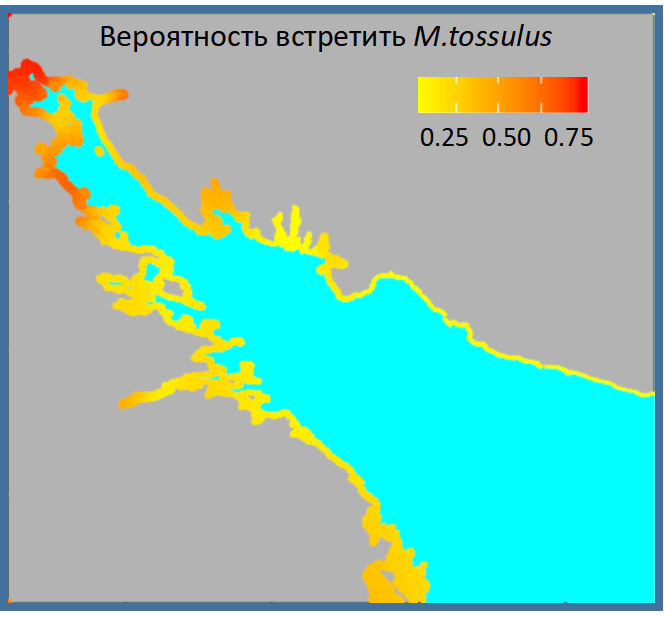
\includegraphics[width=0.7\linewidth]{Mytred_distr.png}
			\captionof{figure}{\color{Green} Распределение видов мидий по акватори Кандалакшского залива.}
			\label{Fig_distred}
		\end{center}\vspace{0.5cm}
\end{minipage}


		\color{DarkSlateGray} % DarkSlateGray color for the rest of the content
		
% 
% 
% \vspace{0.5cm}


\subsection*{Идентификация мидий}


%
\begin{minipage}[b]{0.4\linewidth}

Паттерн закладки перламутрового слоя в районе лигамента (морфотип, рис. ~\ref{Figmorph}) может являться надежным маркером видов \citep{katolikova2016genetic}.   

\begin{itemize}
  \item E-морфотип мидии морфологически близкие к \emph{M.edulis} 
  \item  T-морфотип мидии морфологически близкие к \emph{M.trossulus}
\end{itemize}
 

\end{minipage}\hspace{1cm}
%
\begin{minipage}[t]{0.5\linewidth}
	\begin{center} 
			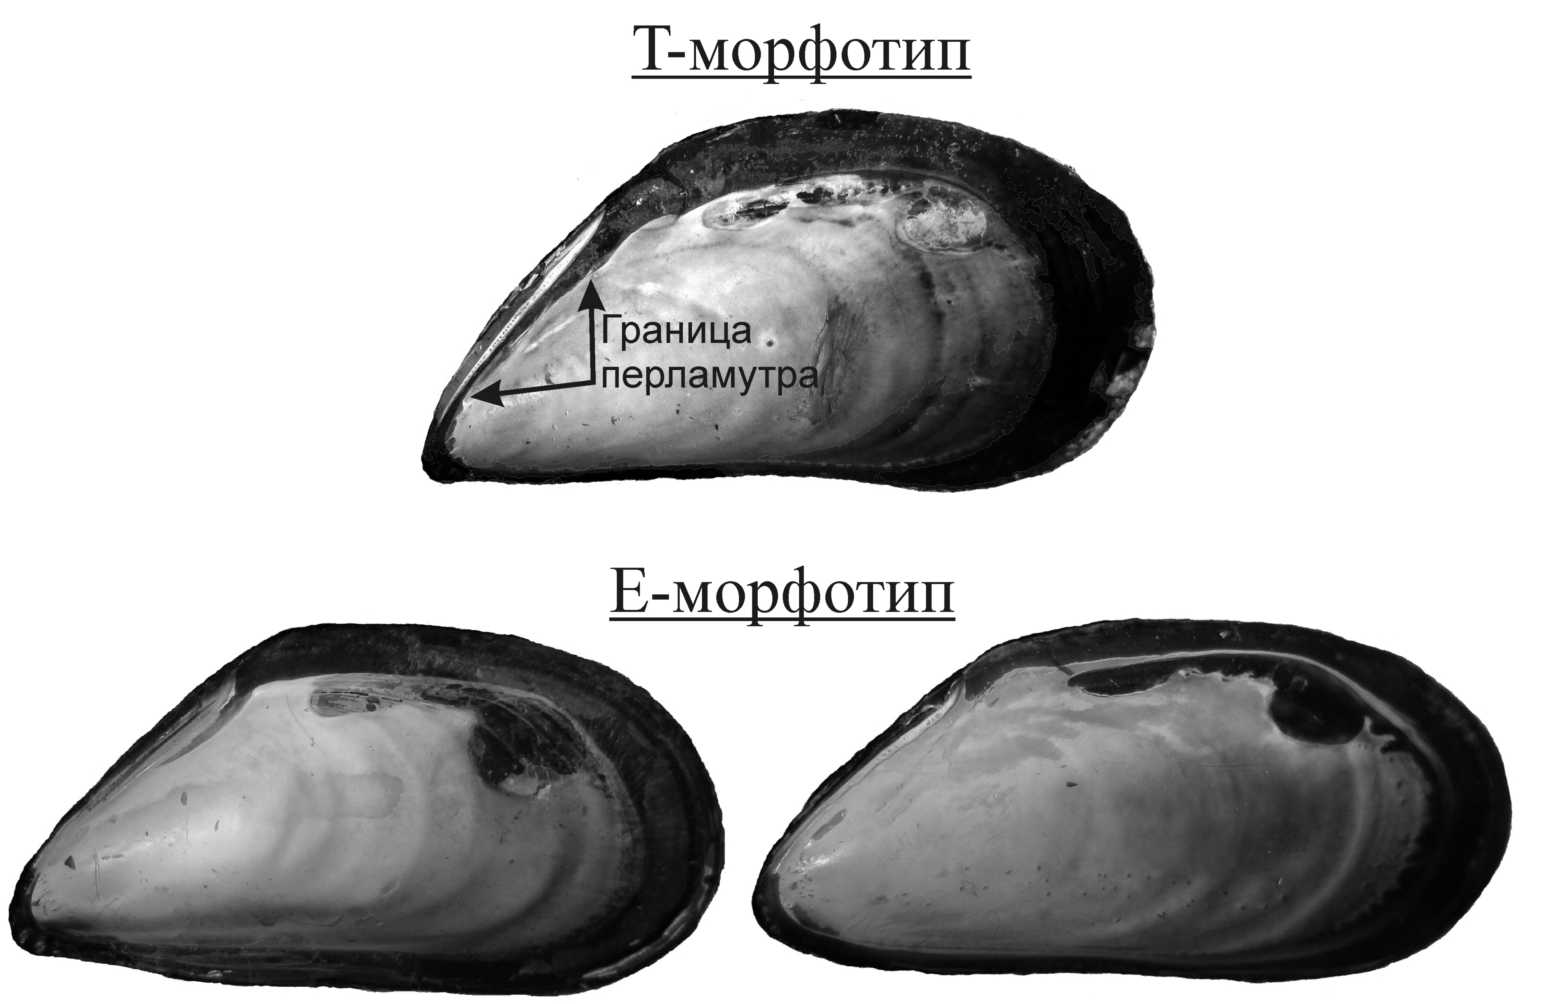
\includegraphics[width=0.6\linewidth]{Morphotypes1.jpg}
			\captionof{figure}{\color{Green} Два морфотипа мидий, различающиеся по паттерну закладки перламутрового слоя.}
			\label{Figmorph}
		\end{center}\vspace{0.5cm}
\end{minipage}


\end{minipage}
%
\begin{minipage}[t]{0.5\linewidth}

% \vspace{4cm}
\section*{\centering {Материал и методика}}

\subsection*{Отбор проб для анализа влиния морских звезд}

%
\begin{minipage}[t]{0.4\linewidth}
Водолаз размещал рамку на участках дна покрытых мидиями и еще не атакованных звездами (Рис. ~\ref{Fig_Sample}, a 1), на участках покрытых агрегациями мидий  (Рис. ~\ref{Fig_Sample}, a 2) и на участках дна, на которых при визуальном осмотре преобладали мертвые раковины с раскрытыми, но сцепленными створками, но без агрегации морских звезд ((Рис. ~\ref{Fig_Sample}, a 3)). Материал был собран с двух участков, один из которых располагался в неопресненном местообитании (Западная Ряжкова Салма), второй -- в эстуарии реки Лувеньга.
\end{minipage}\hspace{1cm}
%
\begin{minipage}[t]{0.5\linewidth}		
	\begin{center}\vspace{0.1cm}
			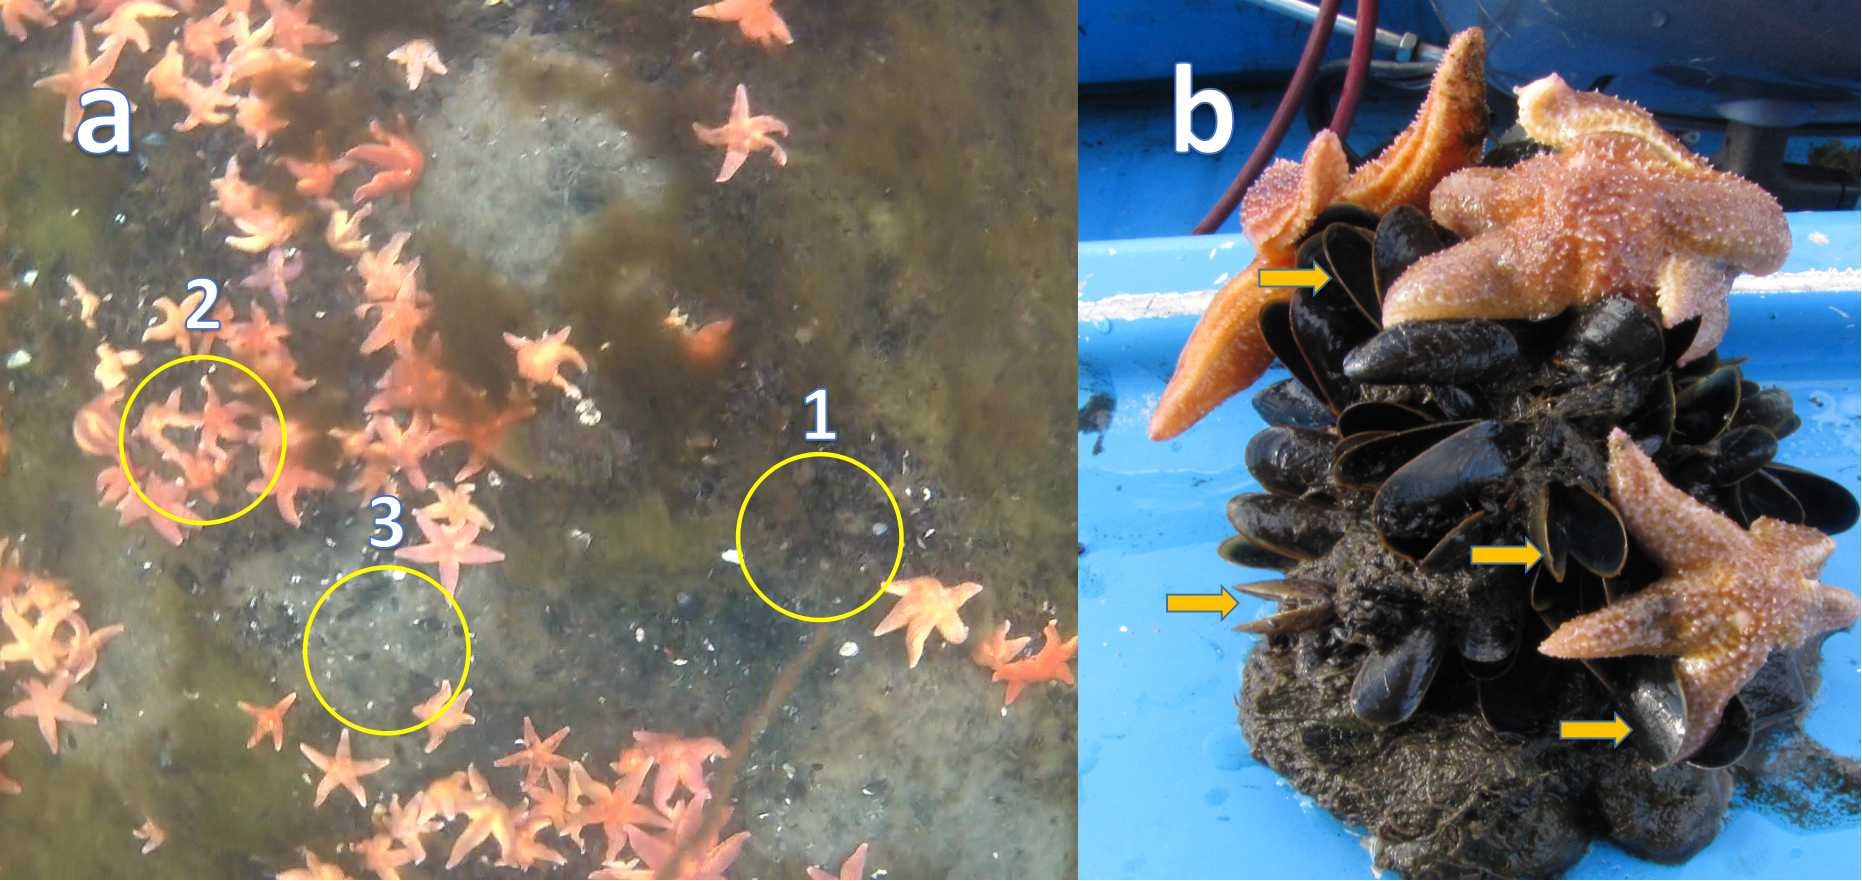
\includegraphics[width=0.8\linewidth]{Samples.jpg}
			\captionof{figure}{\color{Green} Схема отбора проб для оценки влияния морских звезд. (a) Пробы на  поселении мидий не тронутых звездами (1), на скоплениях морских звезд (2) и на скоплениях створок мертвых мидий (3). (b) Агрегация мидий, подвергшаяся атаке морских звезд. Стрелками отмечены съеденные моллюски.}
			\label{Fig_Sample}
		\end{center}
\end{minipage}\hspace{0.5cm}



\subsection*{Отбор проб для анализа влиния кулков-сорок}

%
\begin{minipage}[t]{0.4\linewidth}
На 5 литоральных мидиевых банках, где по результатам многолетних наблюдений постоянно кормились кулики-сороки, был проведен учет живых и съеденных моллюсков. Съеденными считали мертвых мидий, створки которых были соеденены лигаметом, а на внутренней поверхности раковины присутствовали остатки мягких тканей (мантия, мускул замыкатель).  
\end{minipage}\hspace{1cm}
%
\begin{minipage}[t]{0.5\linewidth}		
	\begin{center}\vspace{0.1cm}
			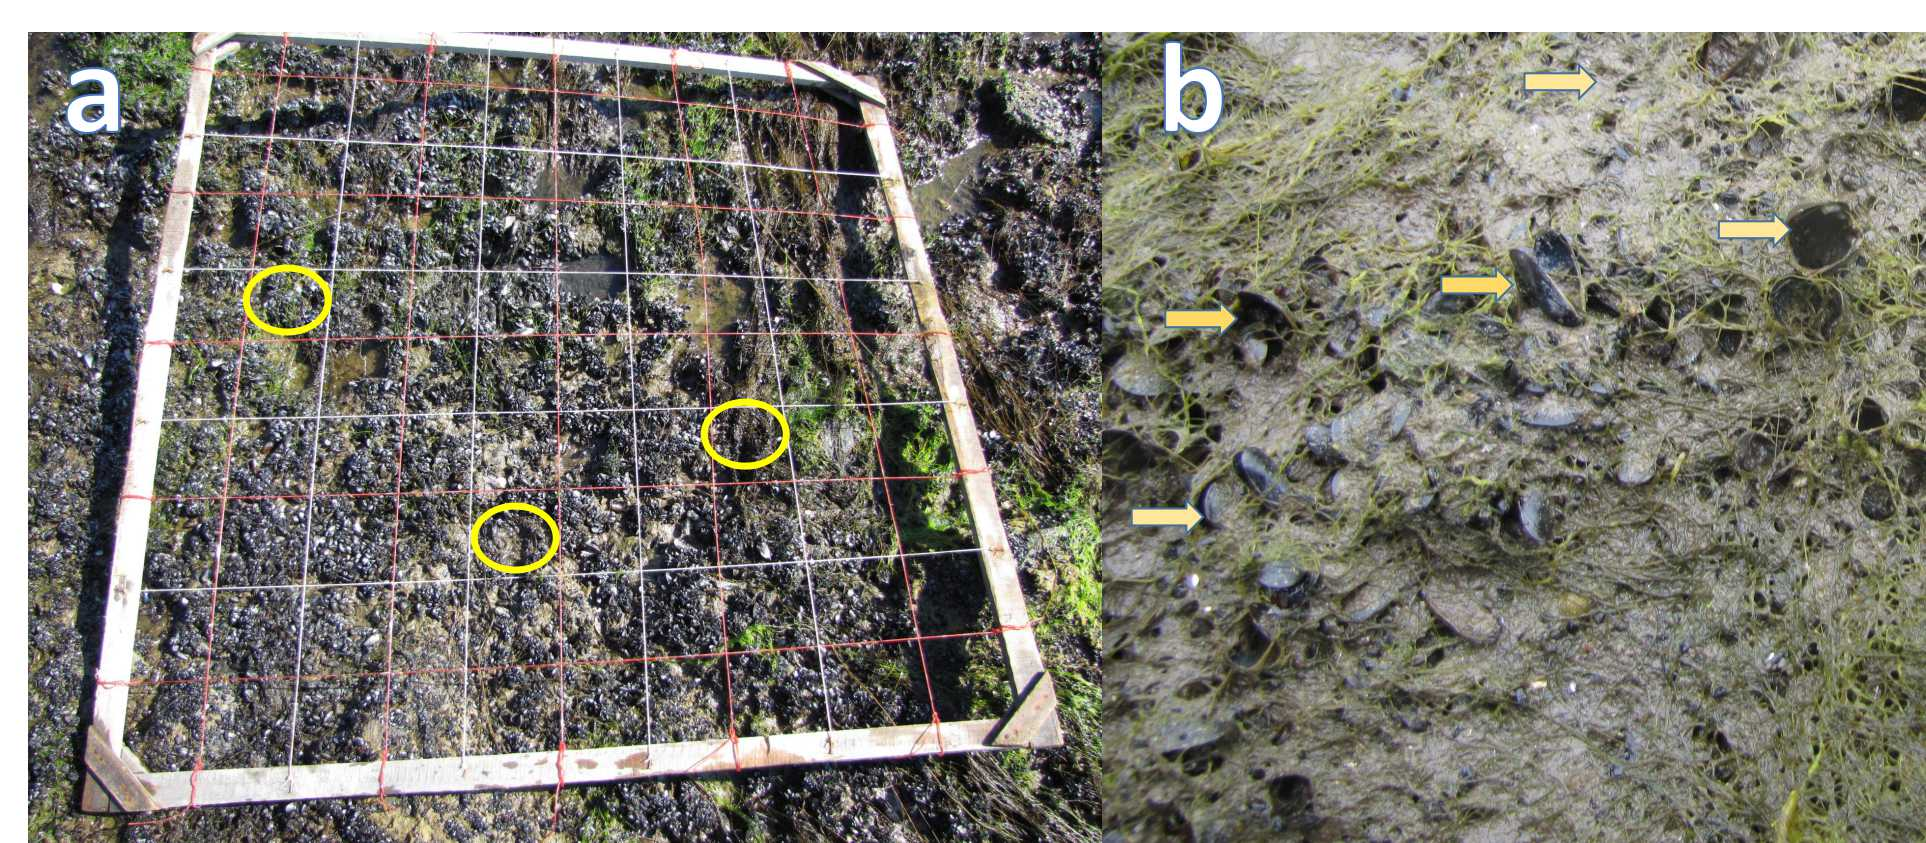
\includegraphics[width=0.8\linewidth]{Samples_oystercatchers.jpg}
			\captionof{figure}{\color{Green} Схема отбора проб для оценки влияния кулков-сорок.(a) Учетна площадка на мидиевой банке. (b) Место кормления кулика-сороки. Стрелками помечены съеденные мидии.}
			\label{Fig_setup}
		\end{center}
\end{minipage}

\vspace{0.5cm}


Для дальнейшего анализа раковины живых и мертвых мидий были измерены (далее использовали только моллюсков с диной рковины более 10 мм) и них был определен морфотип.  



\end{minipage}


% \end{multicols}







%%%%%%%%%%%%%%%%%%% Результаты %%%%%%%%%%%%%%%%%%%%%%%%%%%%
% \section*{\centering {Результаты}}

\vspace{1cm}


% \begin{multicols}{2}
\begin{minipage}[t]{0.46\linewidth}


\subsection*{\centering{\huge{Влияние морских звезд}}}
		





%
\begin{minipage}[t]{0.46\linewidth}		
	\begin{center}\vspace{0.1cm}
			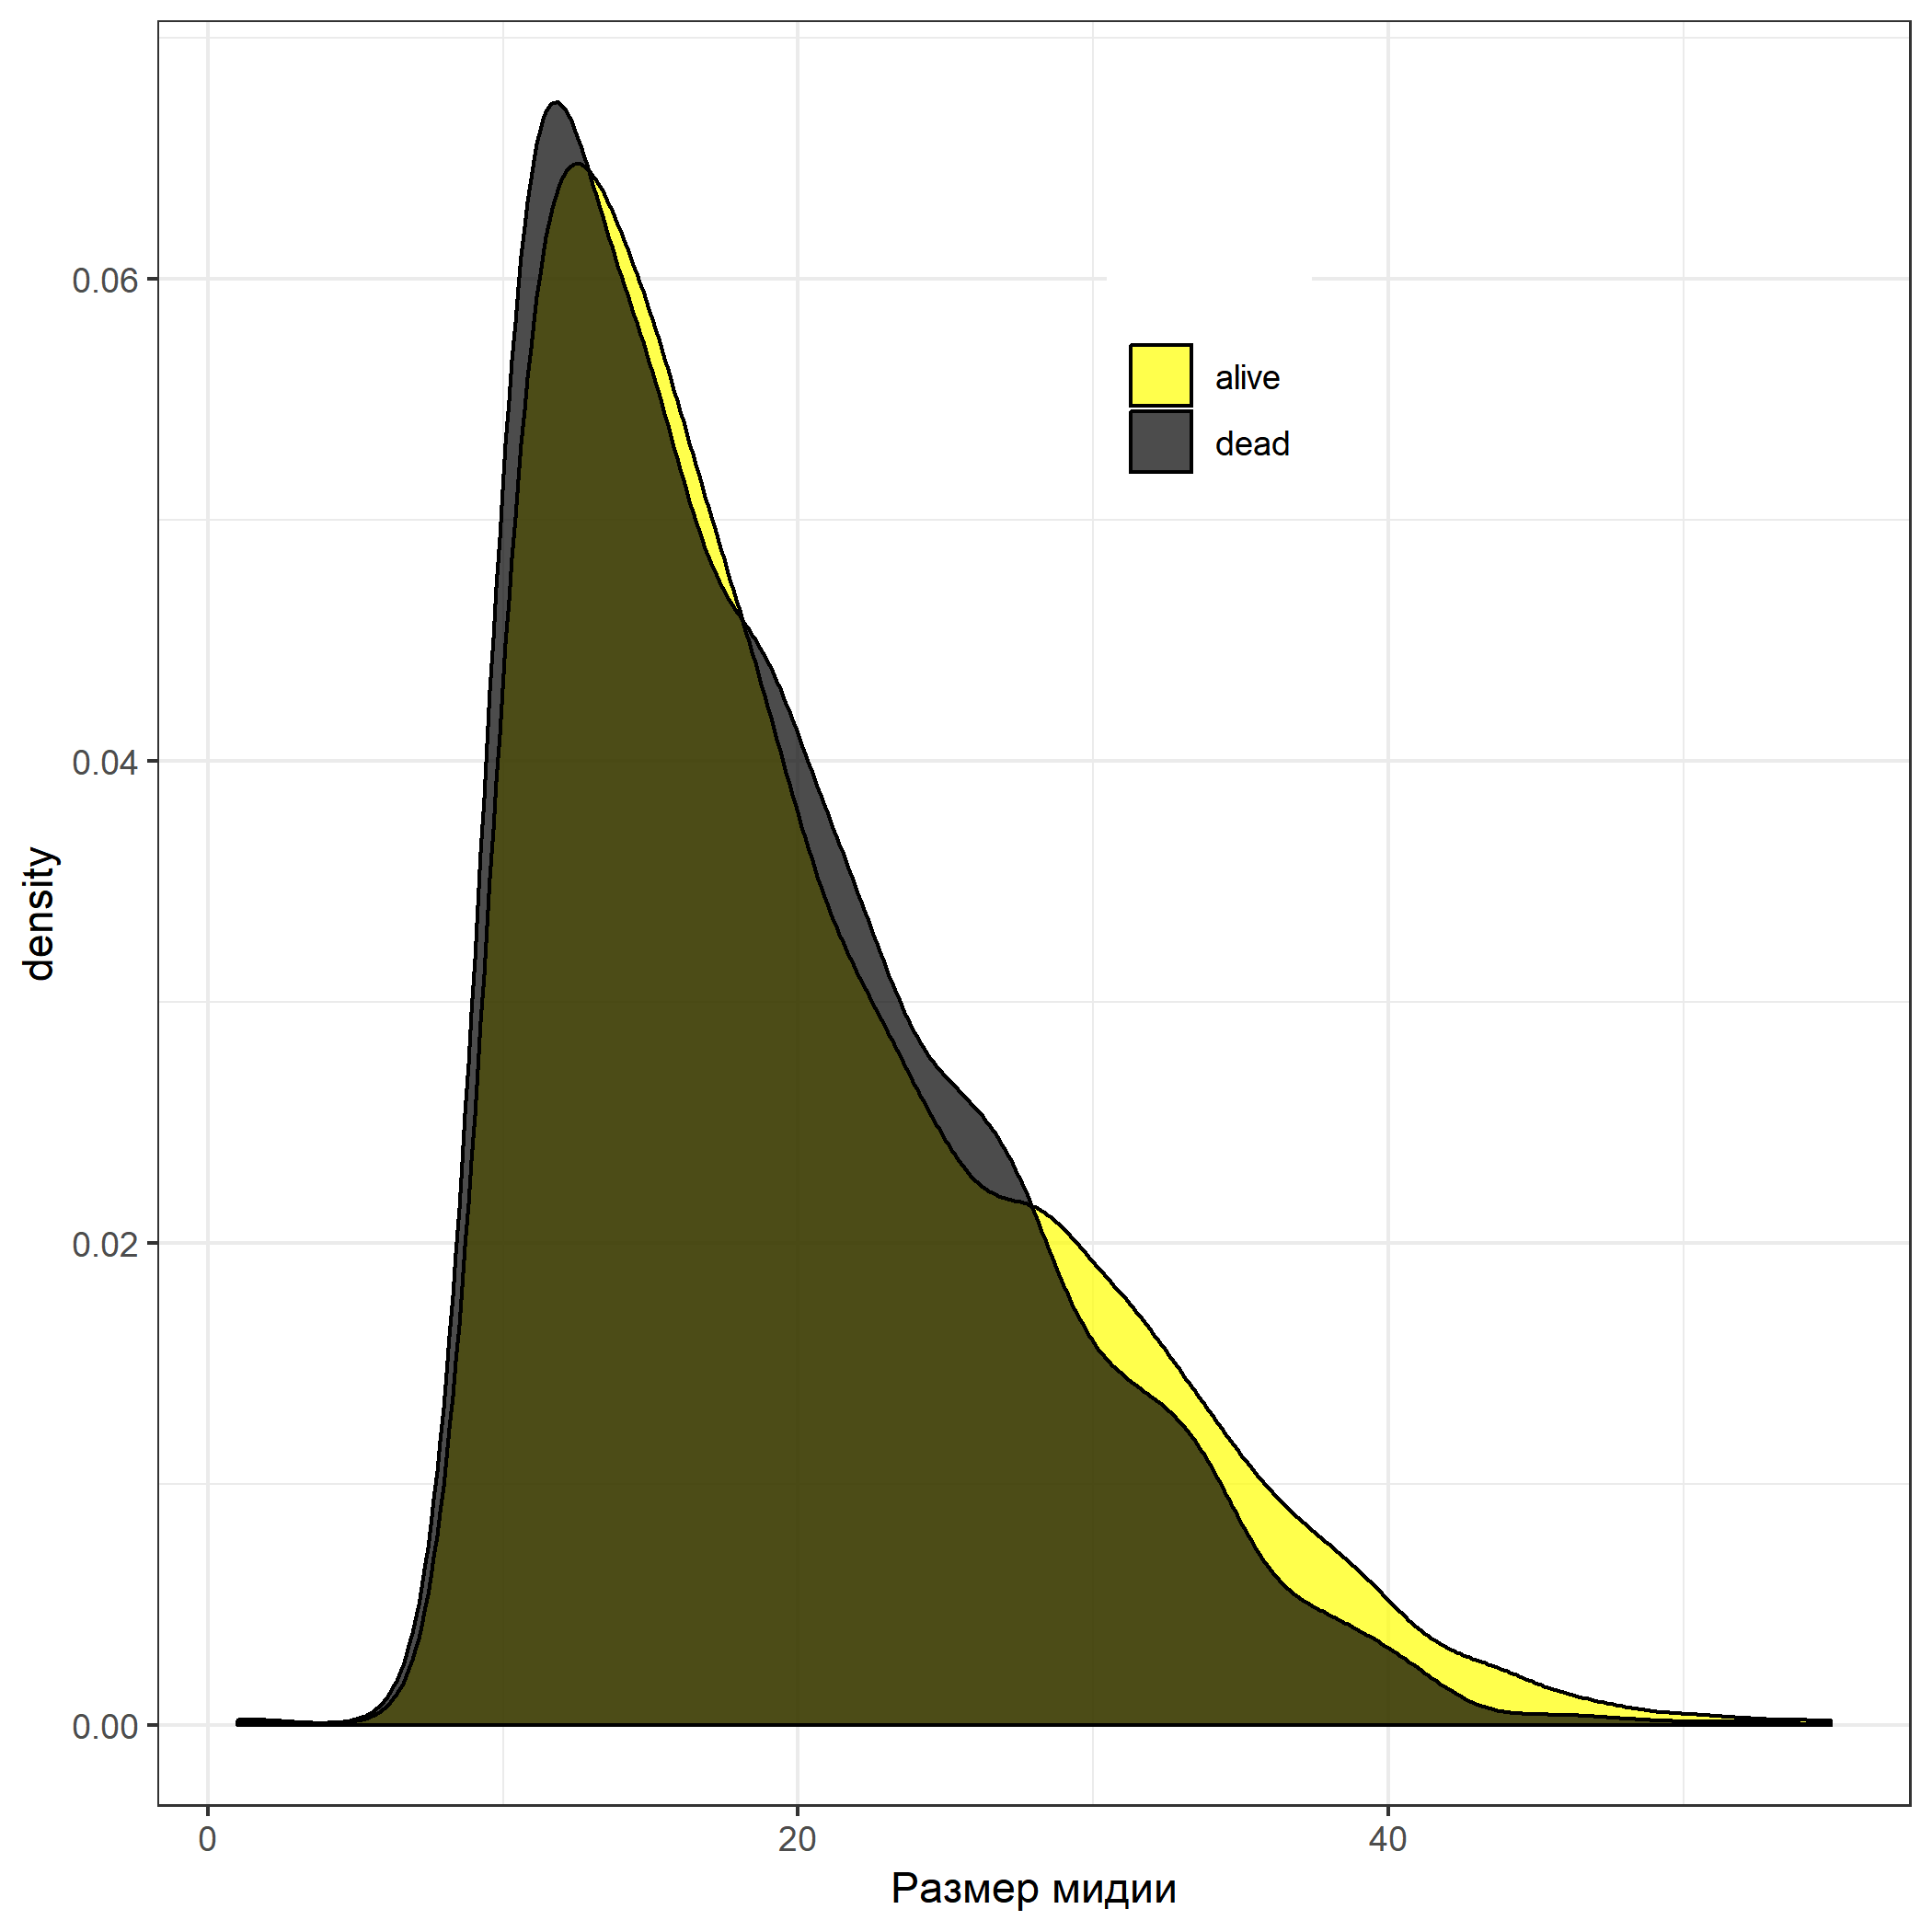
\includegraphics[width=0.9\linewidth]{Size_dist_ast.png}
			\captionof{figure}{\color{Green} Размерная структура живых мидий и мидий, съеденных морскими звездами.}
			\label{Fig_siz_ast}
		\end{center}\vspace{0.5cm}
\end{minipage}\hspace{1cm}
%
\begin{minipage}[t]{0.46\linewidth}		
	\begin{center}\vspace{0.1cm}
			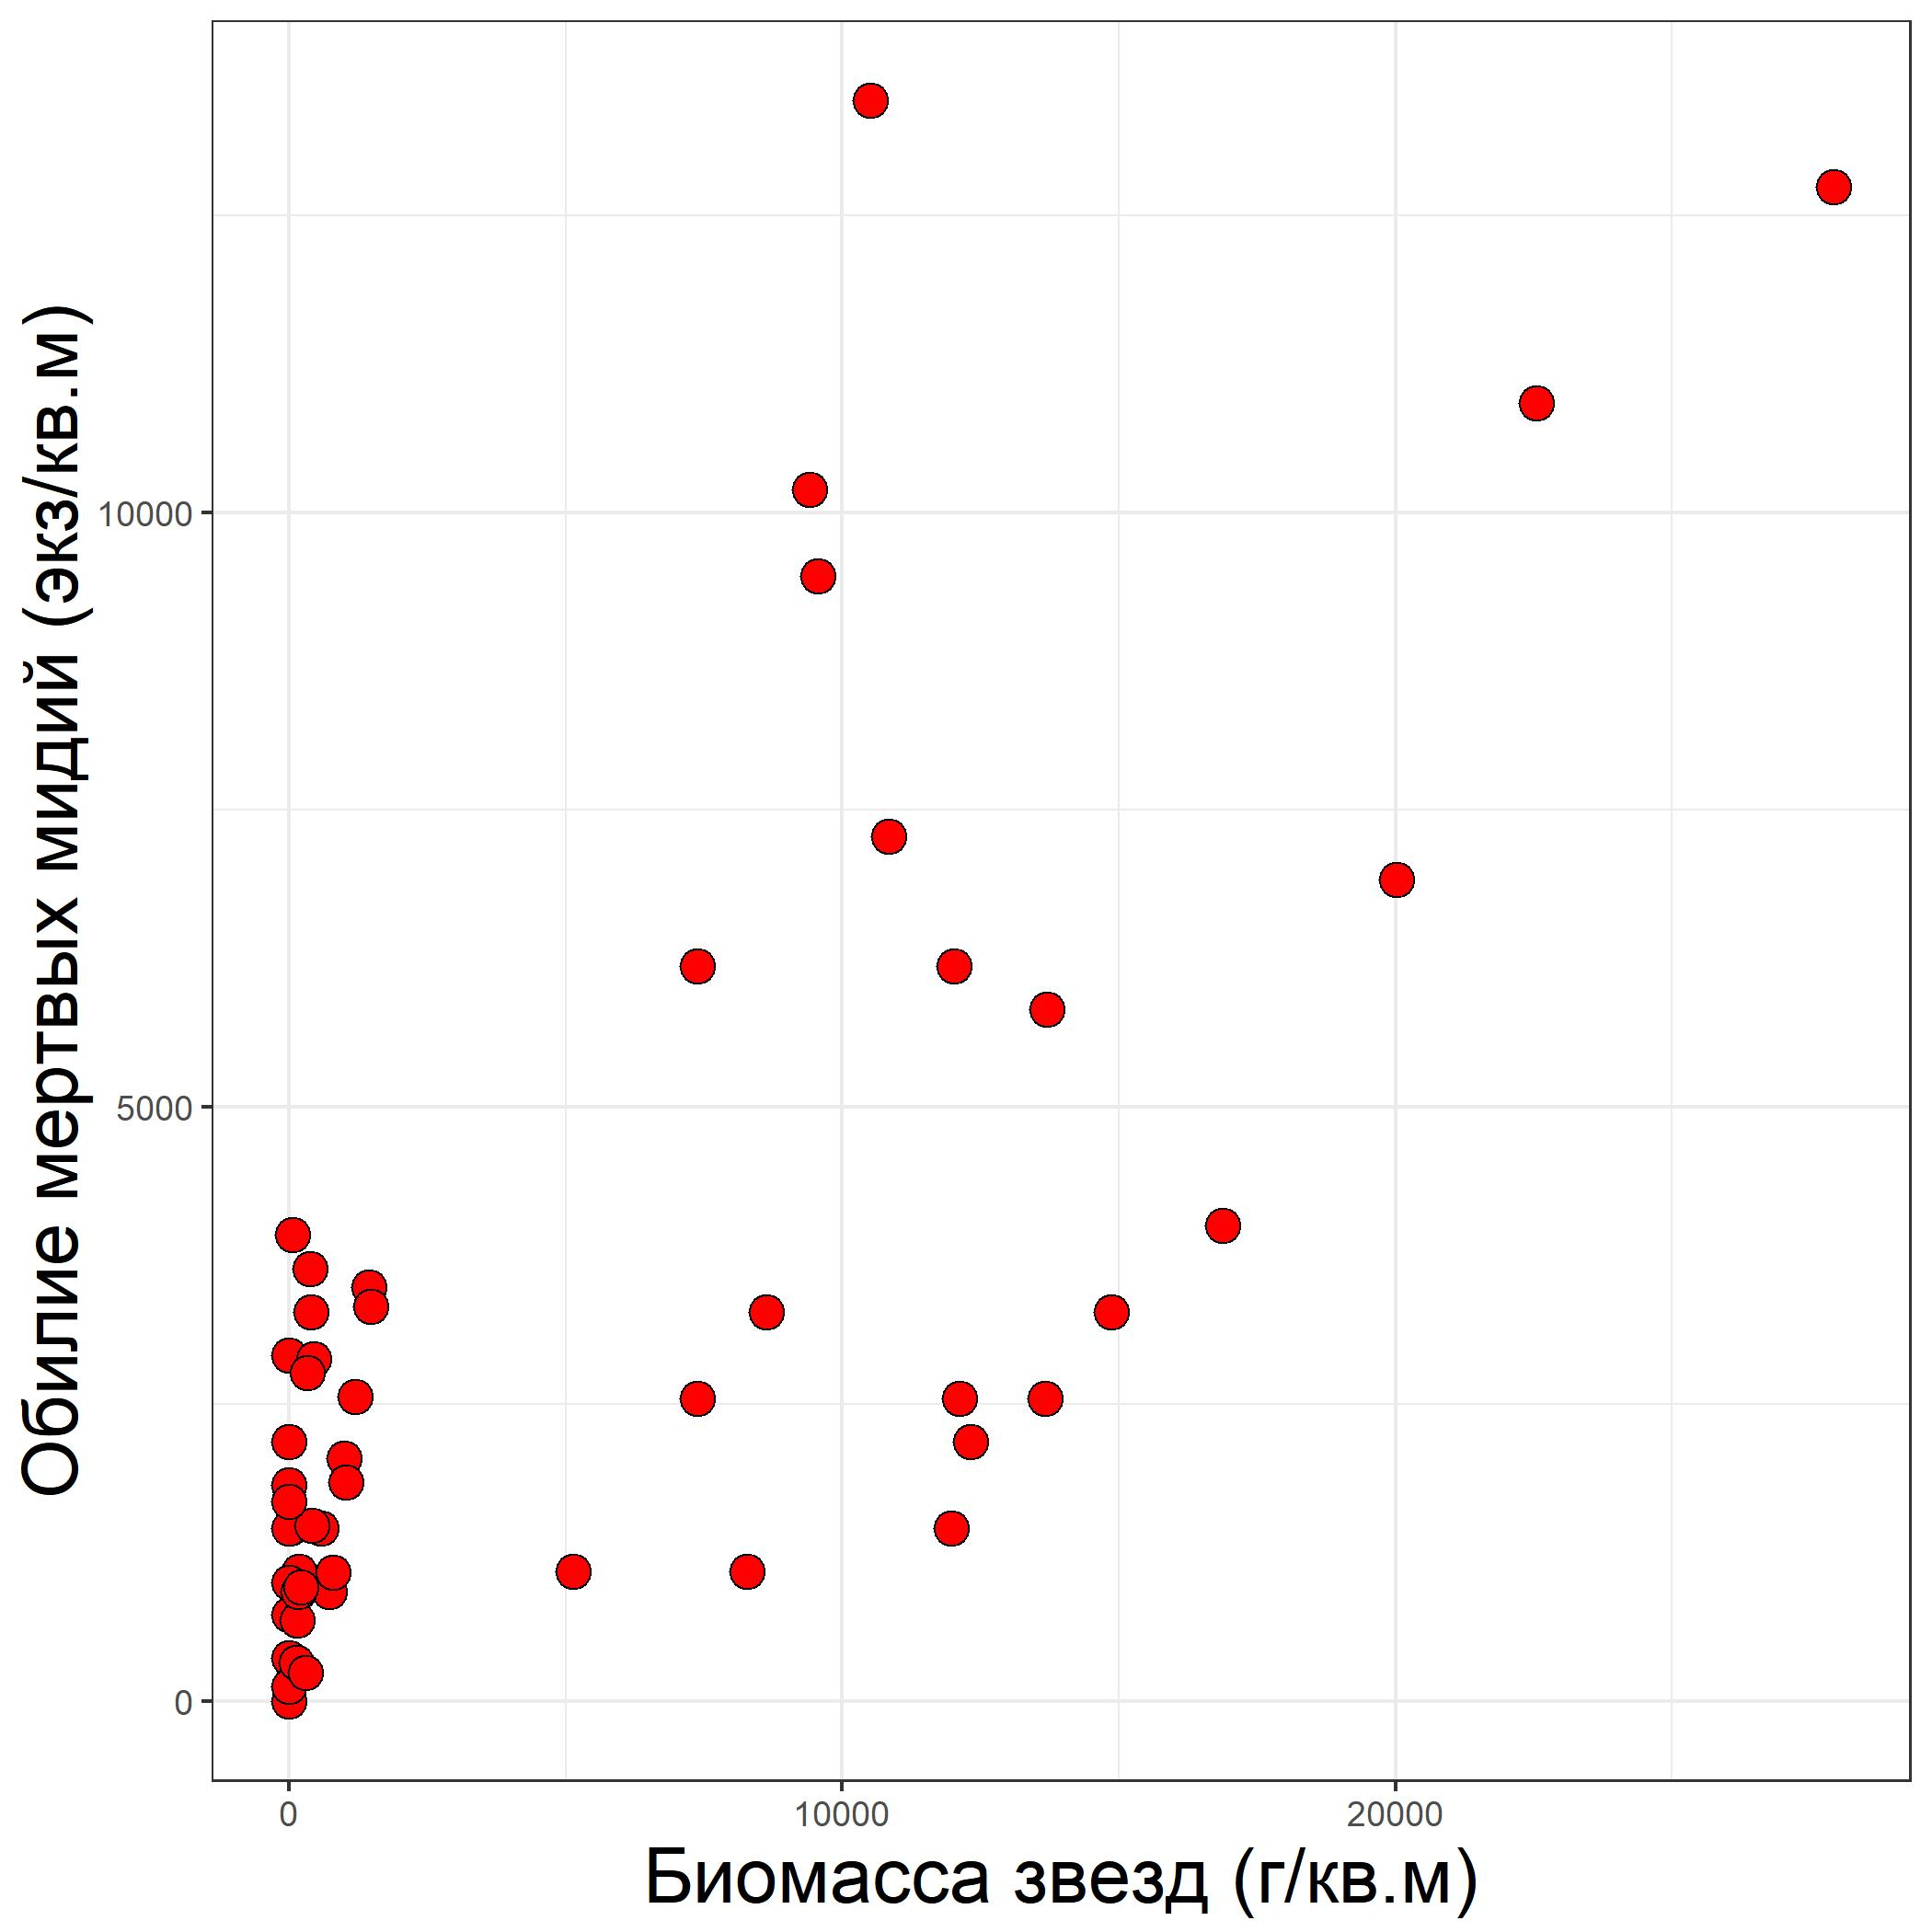
\includegraphics[width=0.9\linewidth]{Baster_N_dead.jpg}
			\captionof{figure}{\color{Green} Зависимость обилия мертвых моллюсков от обилия морских звезд.}
			\label{Baster_Ndead}
		\end{center}\vspace{0.5cm}
\end{minipage}


%
\begin{minipage}[t]{0.46\linewidth}		
	\begin{center}\vspace{0.1cm}
			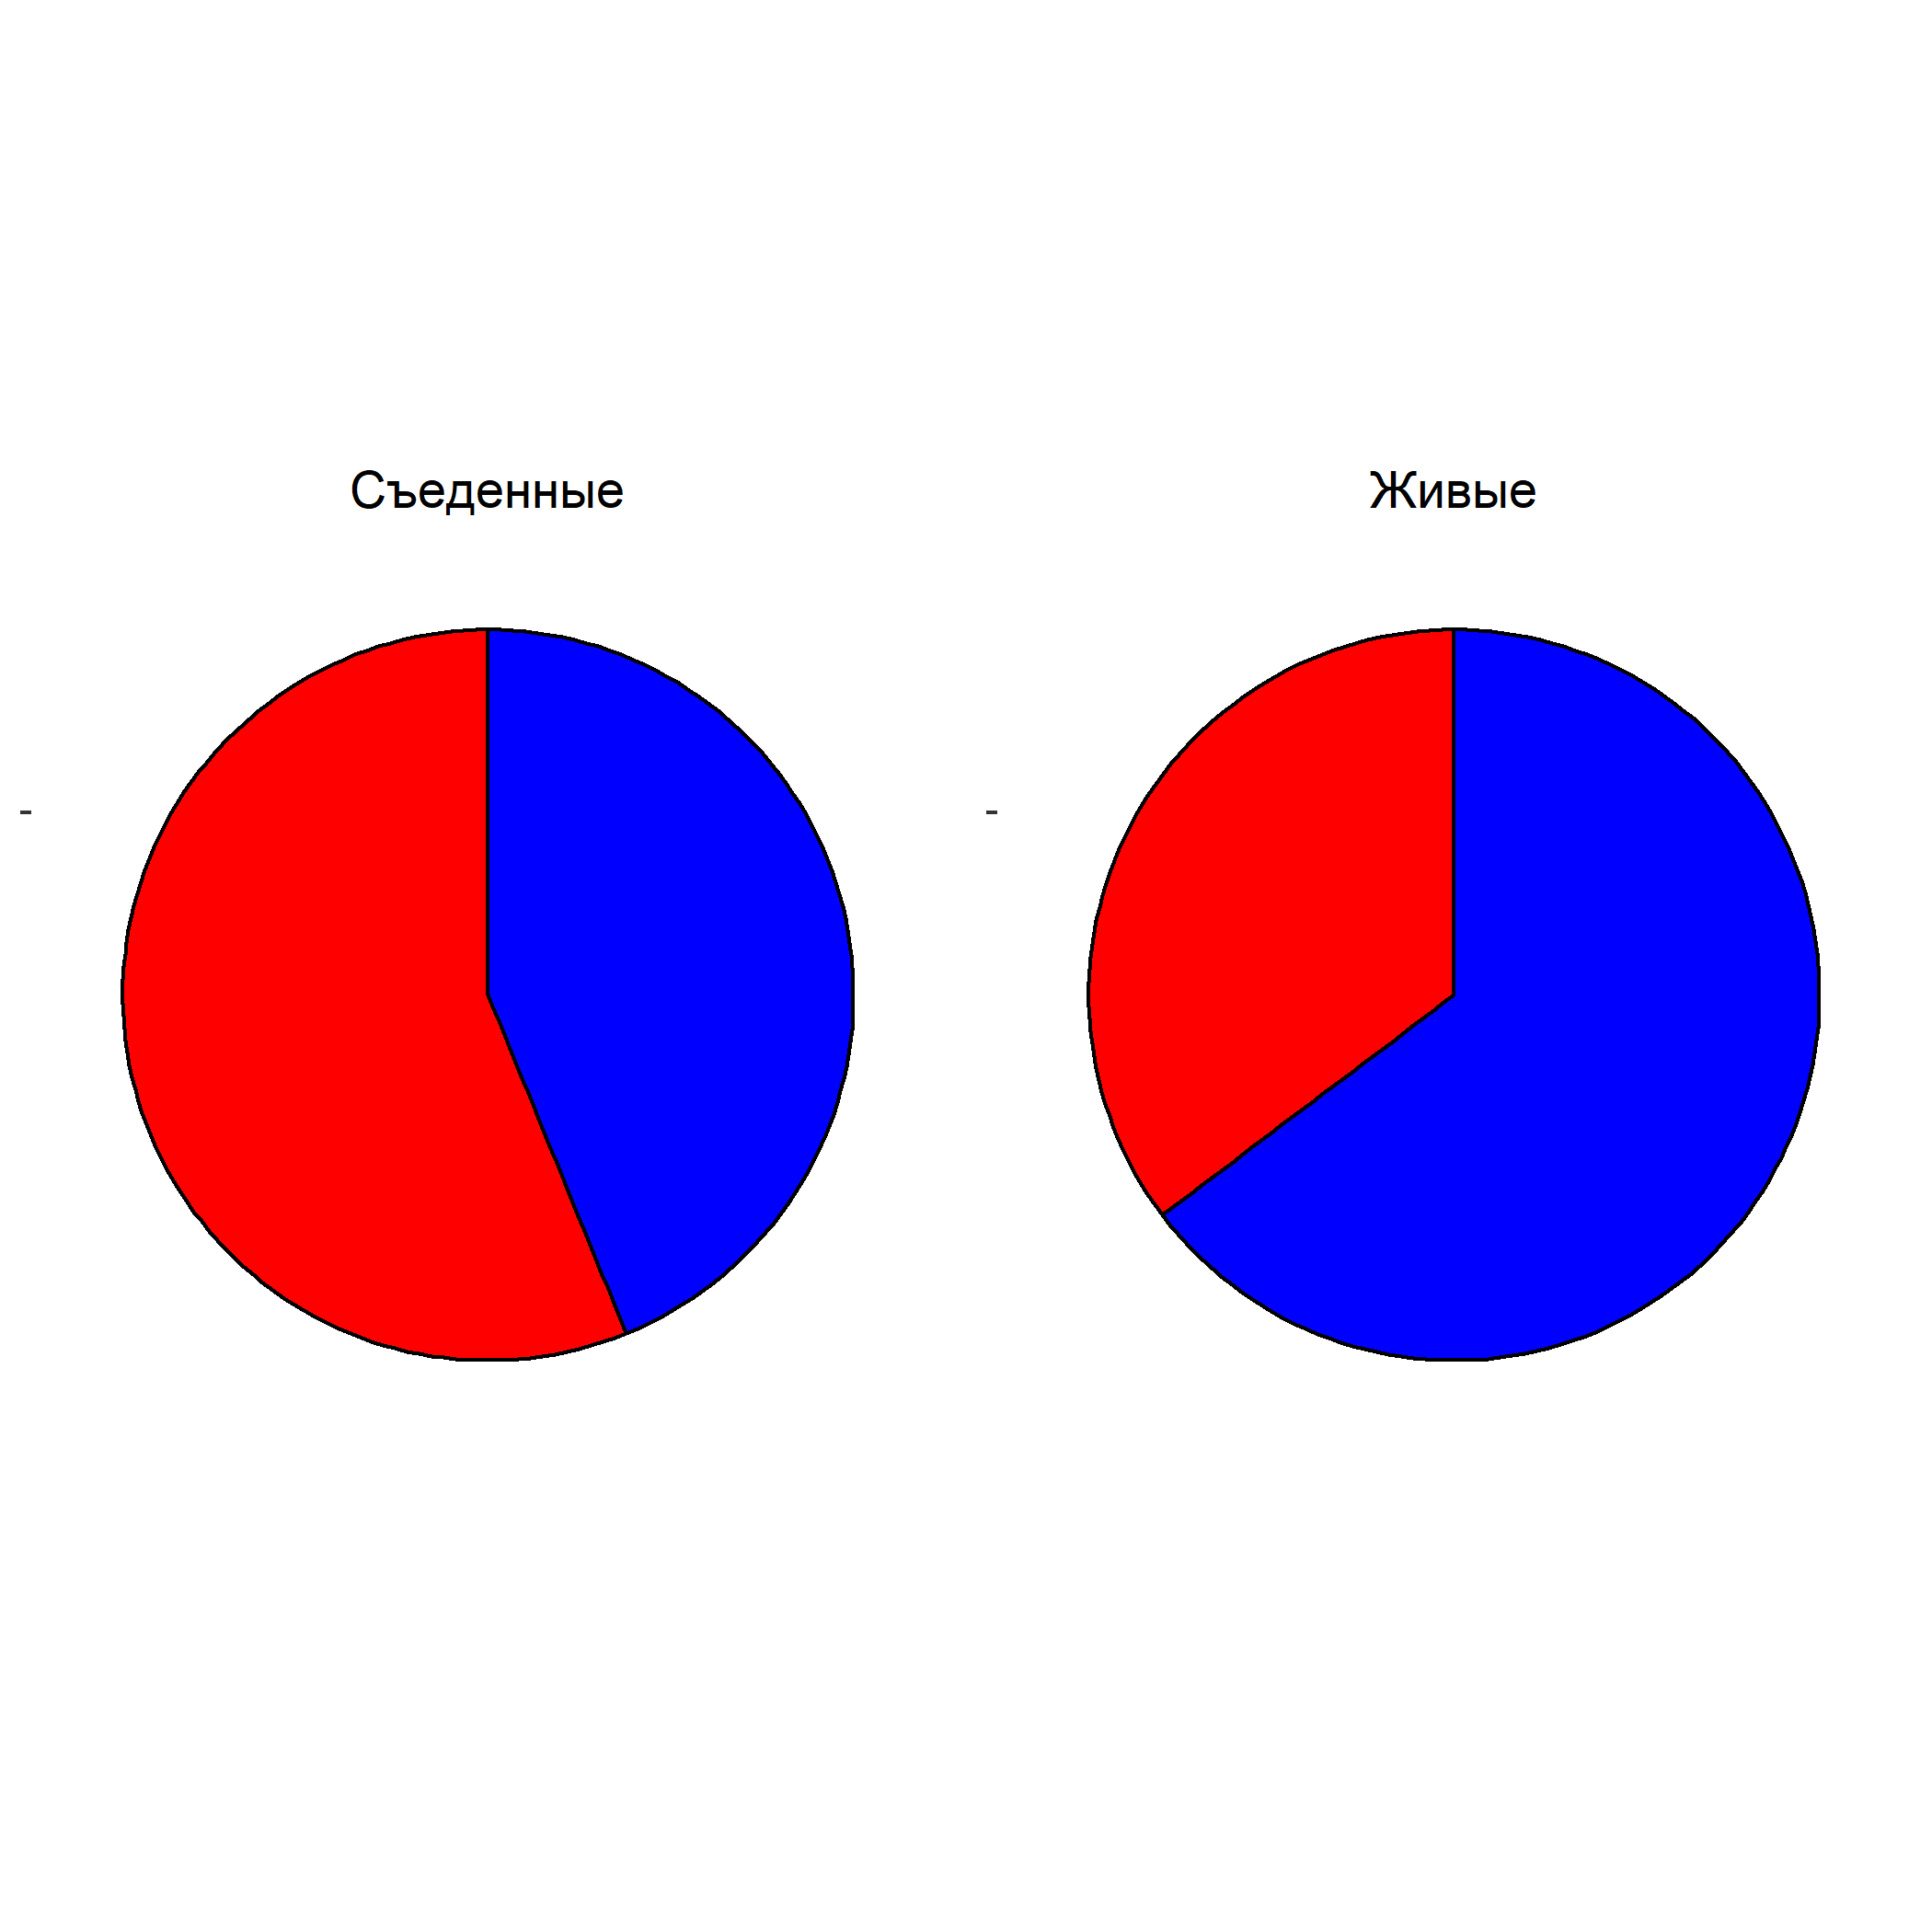
\includegraphics[width=0.9\linewidth]{Pay_charts_aster.png}
			\captionof{figure}{\color{Green} Соотношение численностей Т- (красный сектор) и Е-морфотипов (синий сектор) среди живых и съеденных моллюсков.}
			\label{Fig_pay_chart_aster}
		\end{center}
\end{minipage}\hspace{1cm}
%
\begin{minipage}[t]{0.46\linewidth}		
	\begin{center}\vspace{0.1cm}
			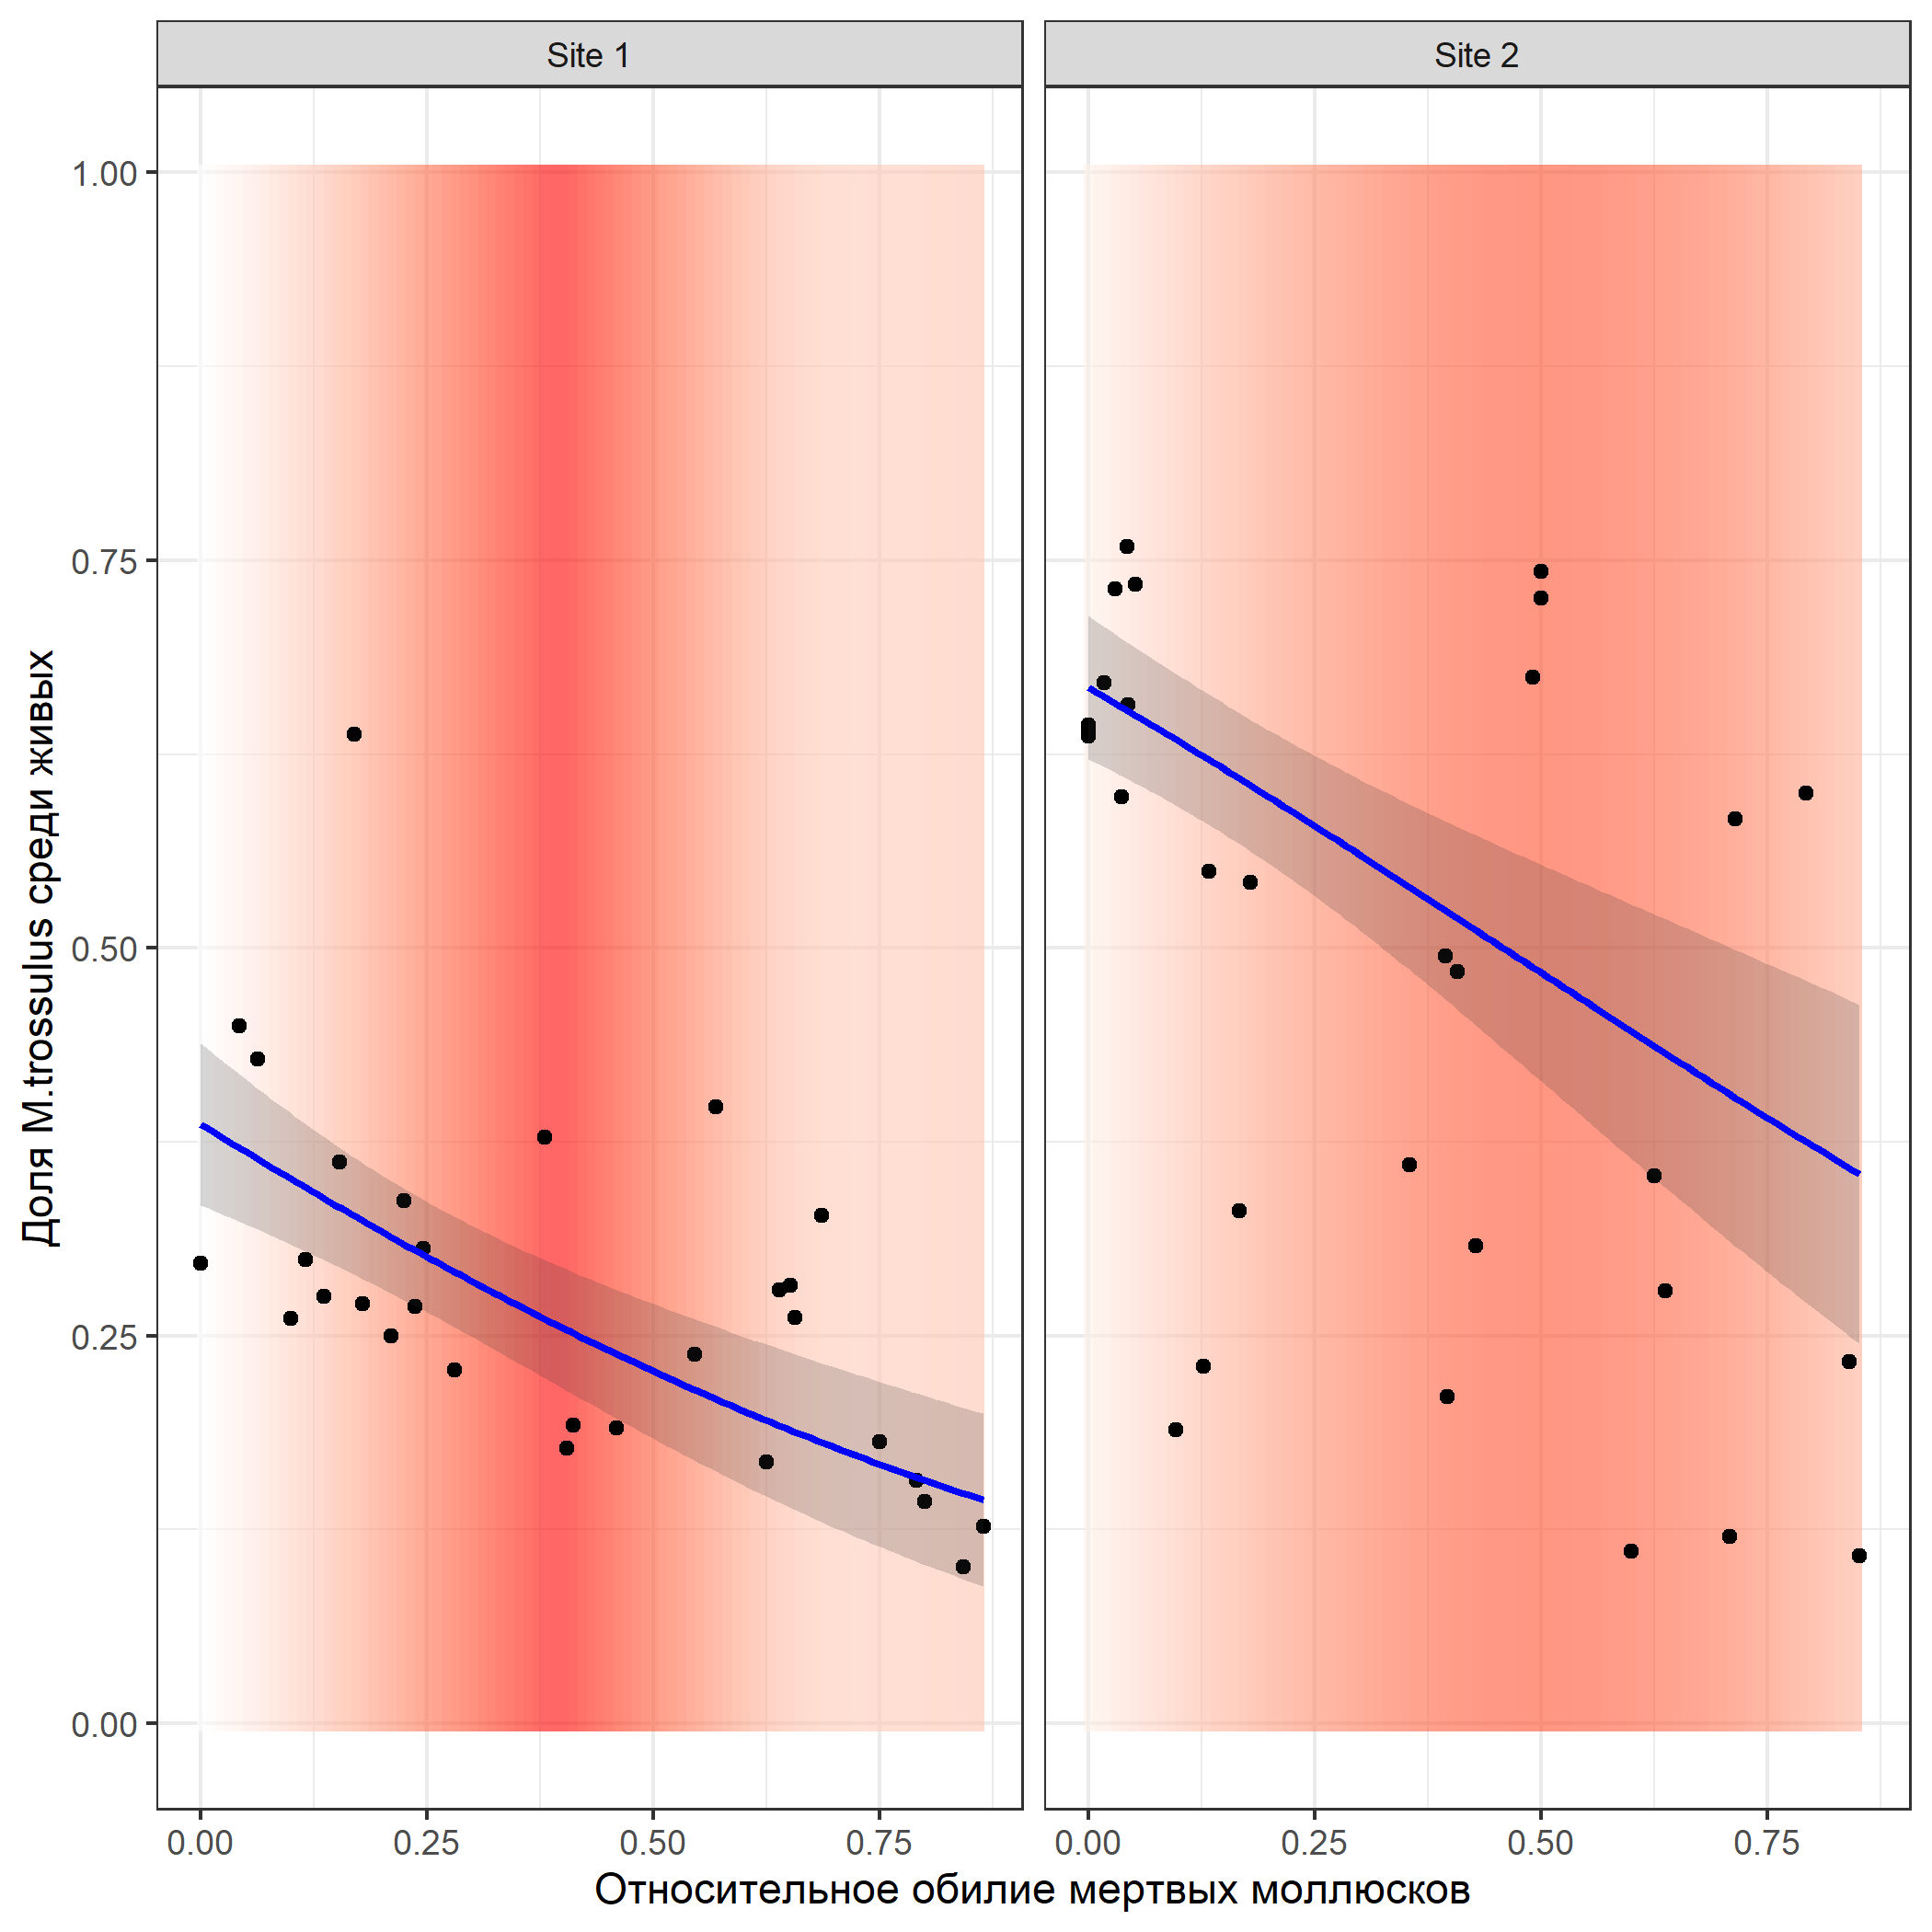
\includegraphics[width=0.9\linewidth]{Prop_dead_Prop_T.png}
			\captionof{figure}{\color{Green} Зависимость доли мидий Т-морфотипа среди живых мидий от обилия съеденных моллюсков. Степень заливк красным пропорциональна биомассе звезд}
			\label{Prop_dead_Prop_T}
		\end{center}
\end{minipage}\vspace{0.5cm}

\vspace{\belowdisplayskip}


Существенных разлчий в размерах съеденных и несъеденных моллюсков не выявлено (рис. \ref{Fig_siz_ast}). 

Обилие мертвых створок (рис. \ref{Baster_Ndead}) возрастает по мере роста обилия звезд. По количеству створок поибших моллюсков можно судить о степени воздействи хищников.  

Доля Т-морфотипа среди съеденных моллюсков (рис.  \ref{Fig_pay_chart_aster}) выше, чем доля таких мидий среди живых особей. Морские звезды предпочитают атаковать мидий Т-морфотипа. 

В обеих точках сбора материала на фоне увеличени доли съеденных мидий наблюдалось падение относительного обилия мидий Т-морфотипа (рис. \ref{Prop_dead_Prop_T}) . Выедание морскими звездами приводит к существенному сокращению относительного обилия \emph{M.trossulus} в смешанном поселении двух видов мидий.

\end{minipage}\vspace{1cm}
%
\begin{minipage}[t]{0.46\linewidth}		

\subsection*{\centering{\huge{Влияние куликов-сорок}}}



%
\begin{minipage}[t]{0.46\linewidth}		
	\begin{center}\vspace{0.1cm}
			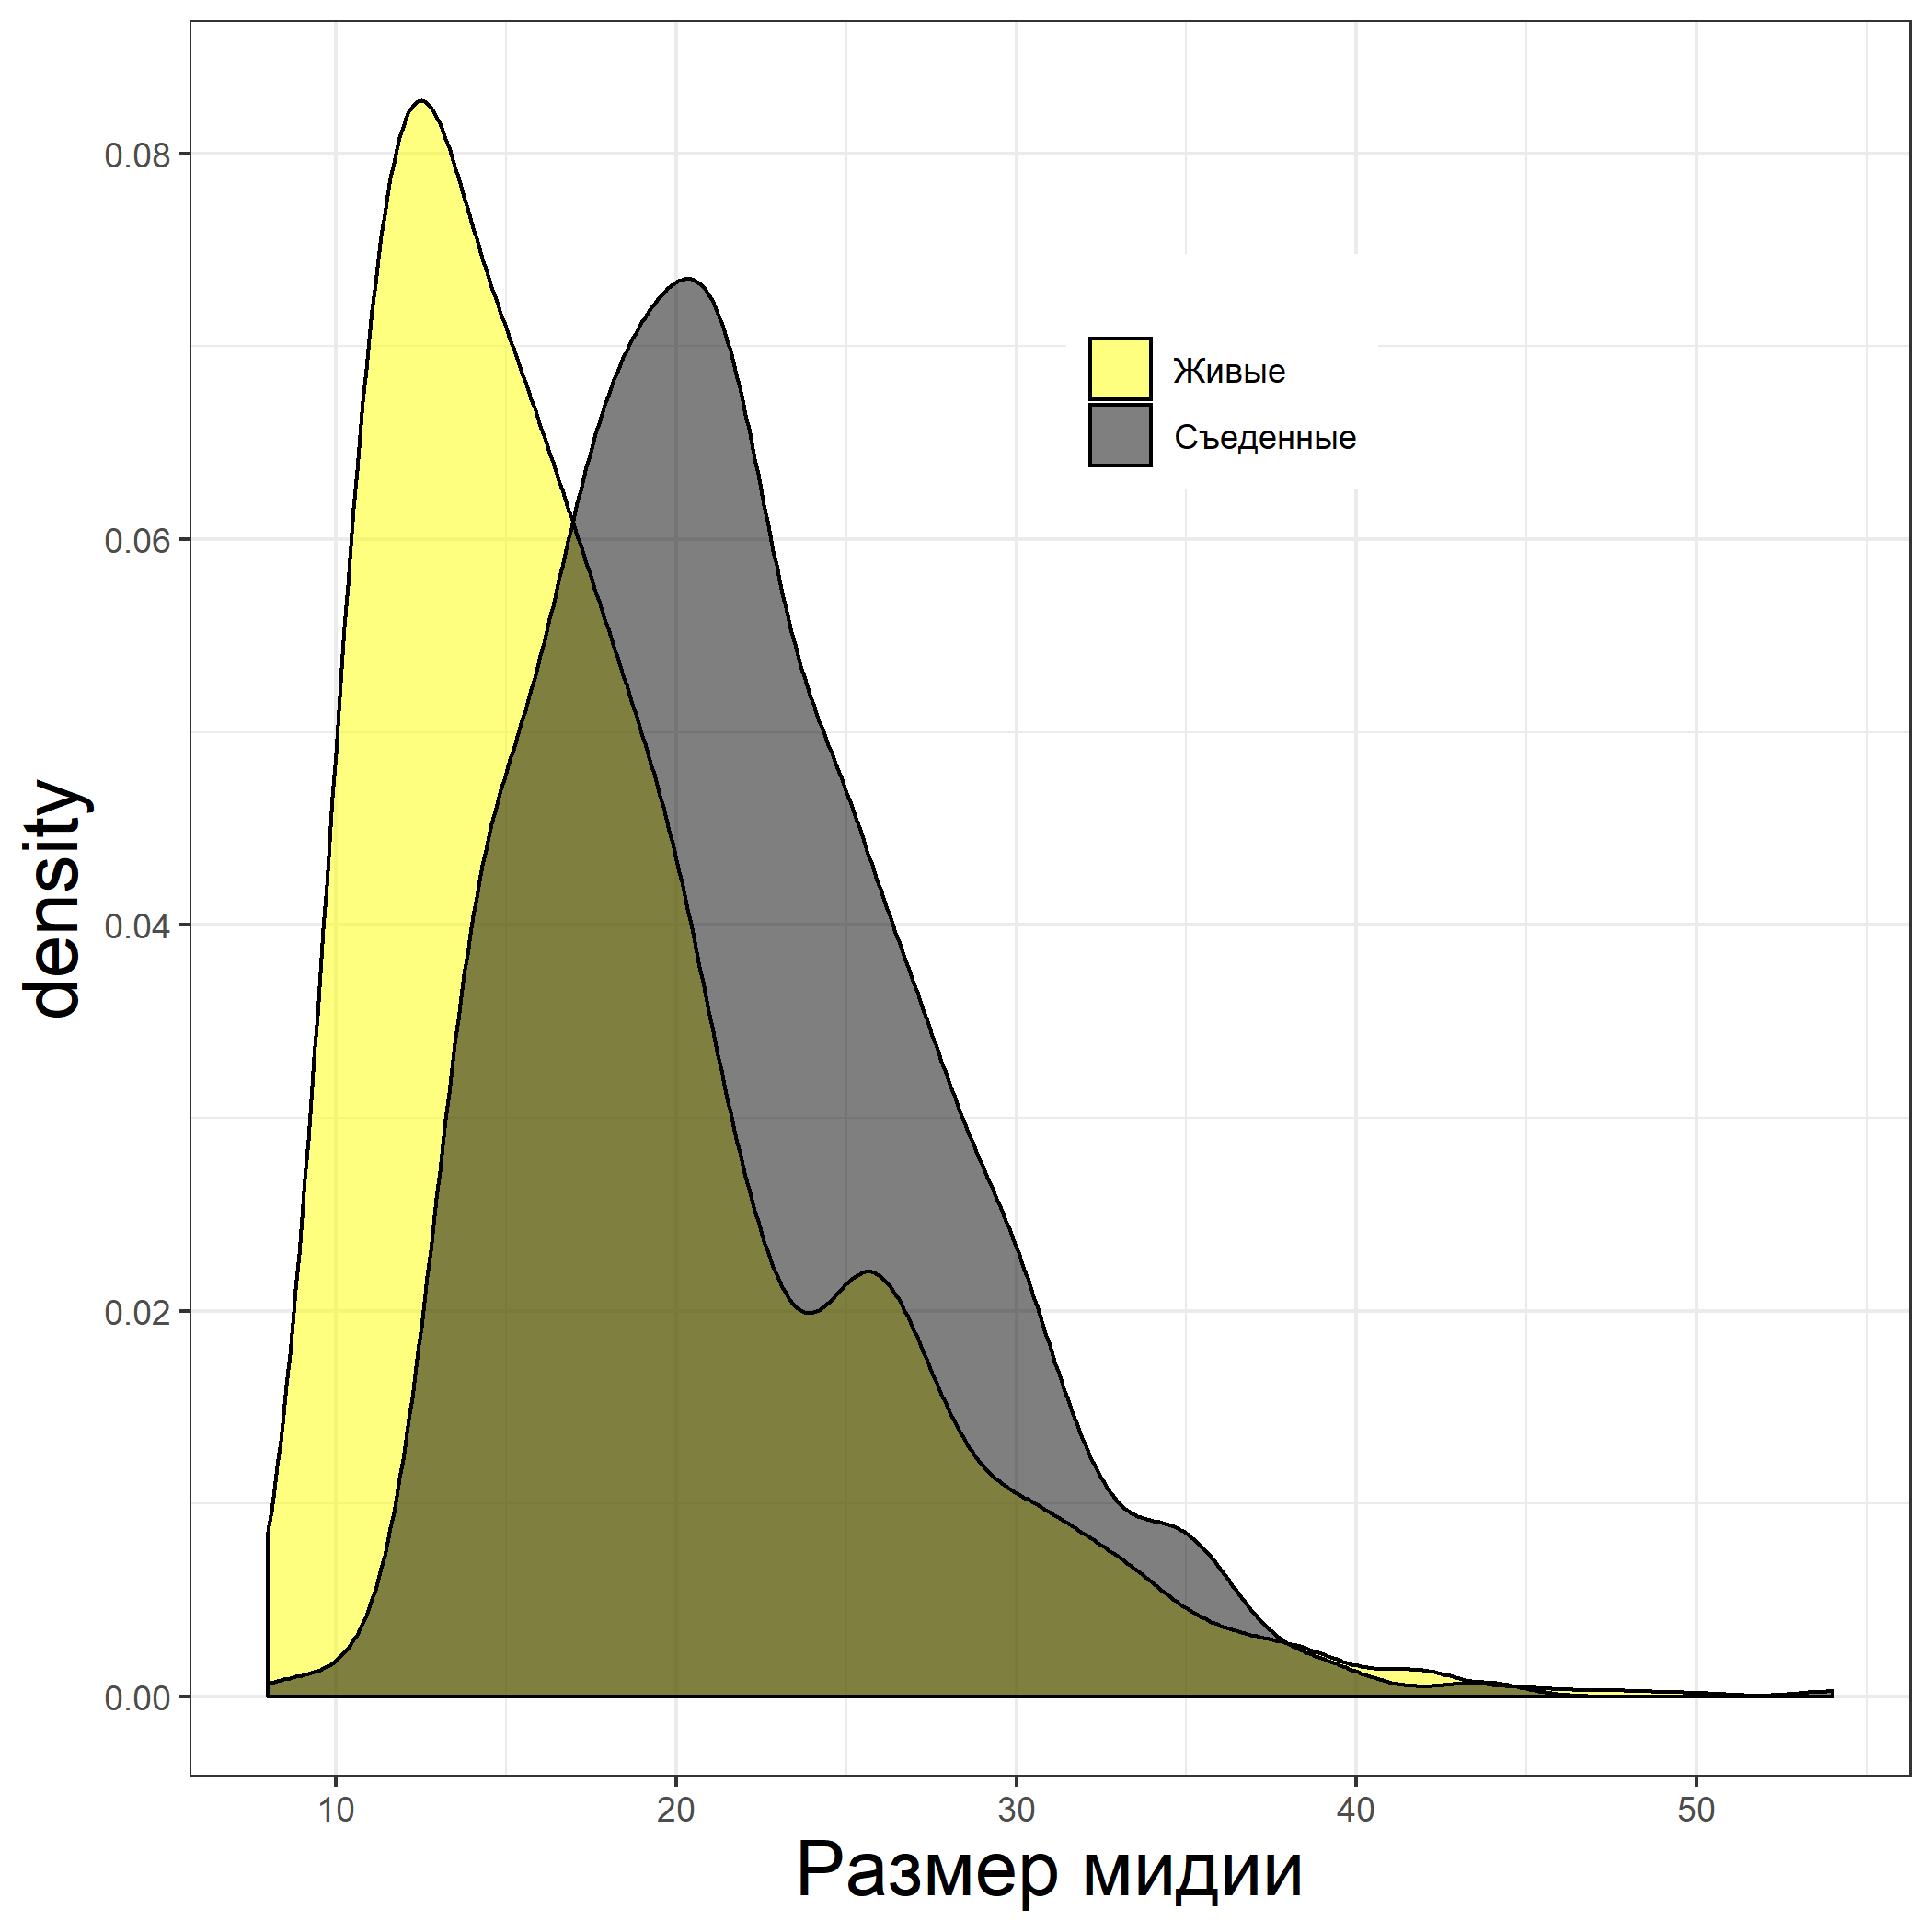
\includegraphics[width=0.9\linewidth]{Size_dist_hem.png}
			\captionof{figure}{\color{Green} Размерная структура живых мидий и мидий, съеденных куликами-сороками.}
			\label{Fig_siz_hem}
		\end{center}\vspace{0.5cm}
\end{minipage}\hspace{2cm}
%
\begin{minipage}[t]{0.46\linewidth}		
	\begin{center}\vspace{0.1cm}
			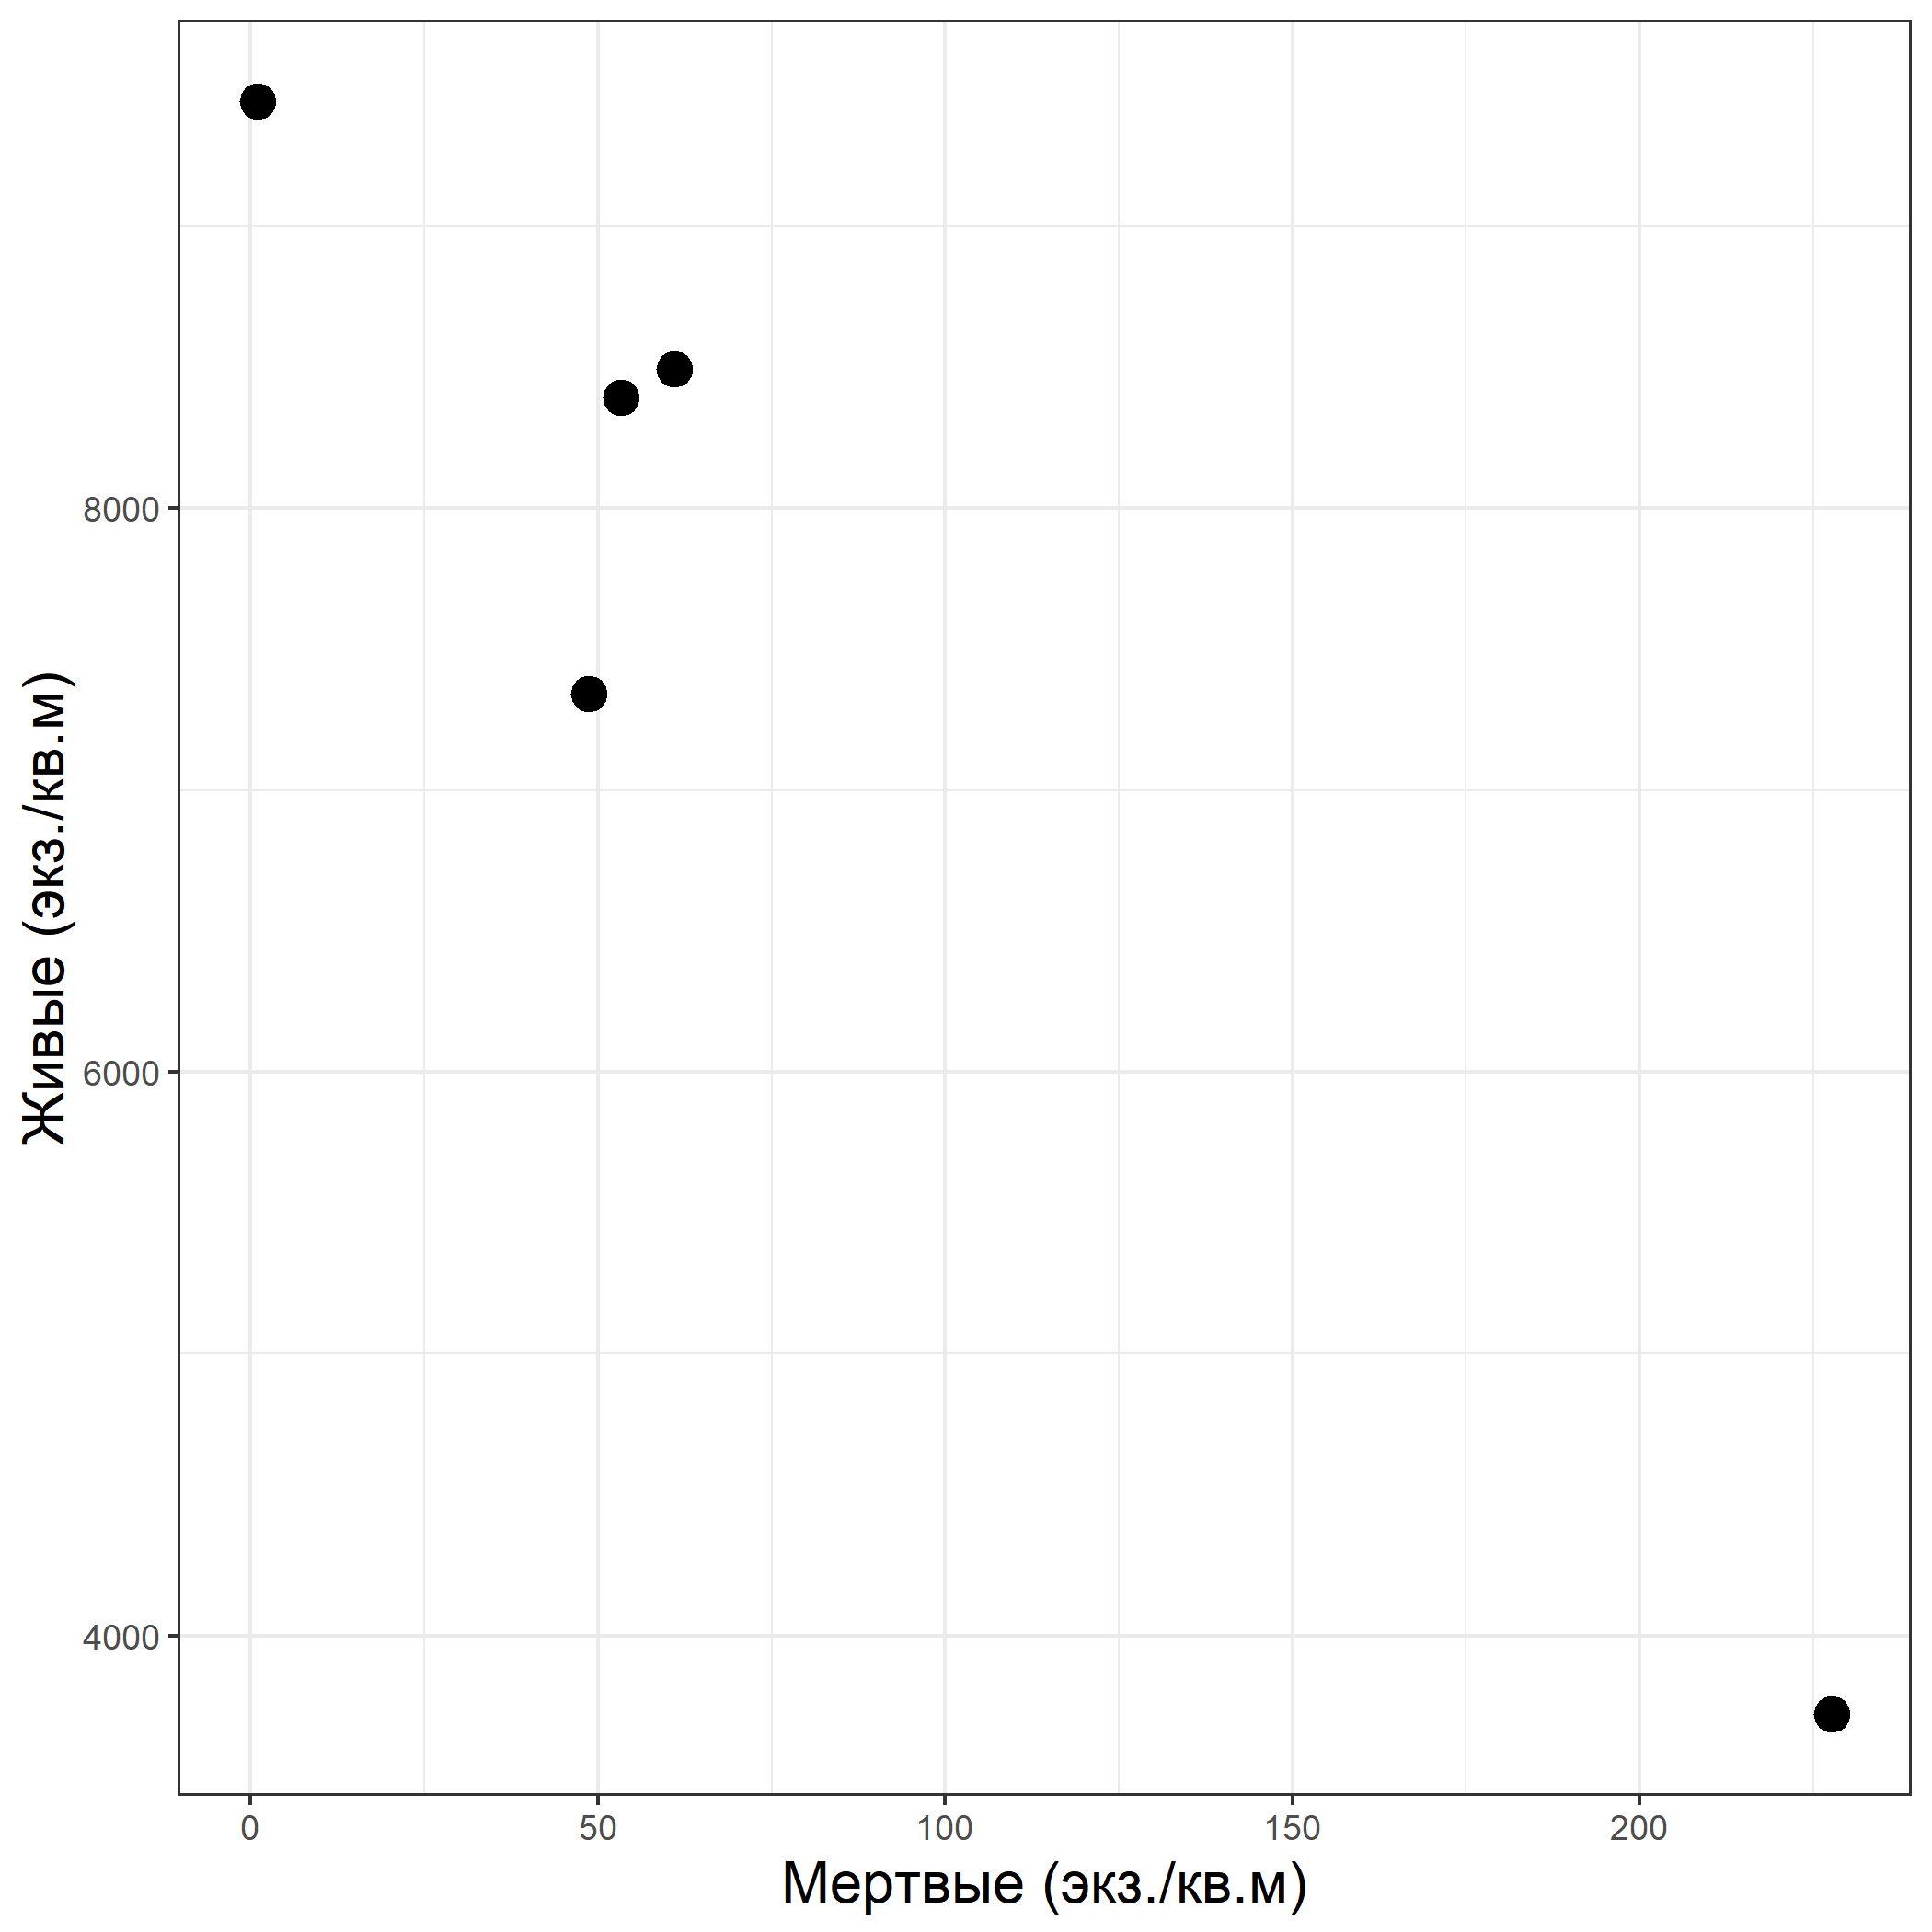
\includegraphics[width=0.9\linewidth]{N_dead_N_alive_hem.png}
			\captionof{figure}{\color{Green} Зависимость обилия живых моллюсков от обилия мертвых створок.}
			\label{Nalive_Ndead_hem}
		\end{center}\vspace{0.5cm}
\end{minipage}


\begin{minipage}[t]{0.46\linewidth}		
	\begin{center}\vspace{0.1cm}
			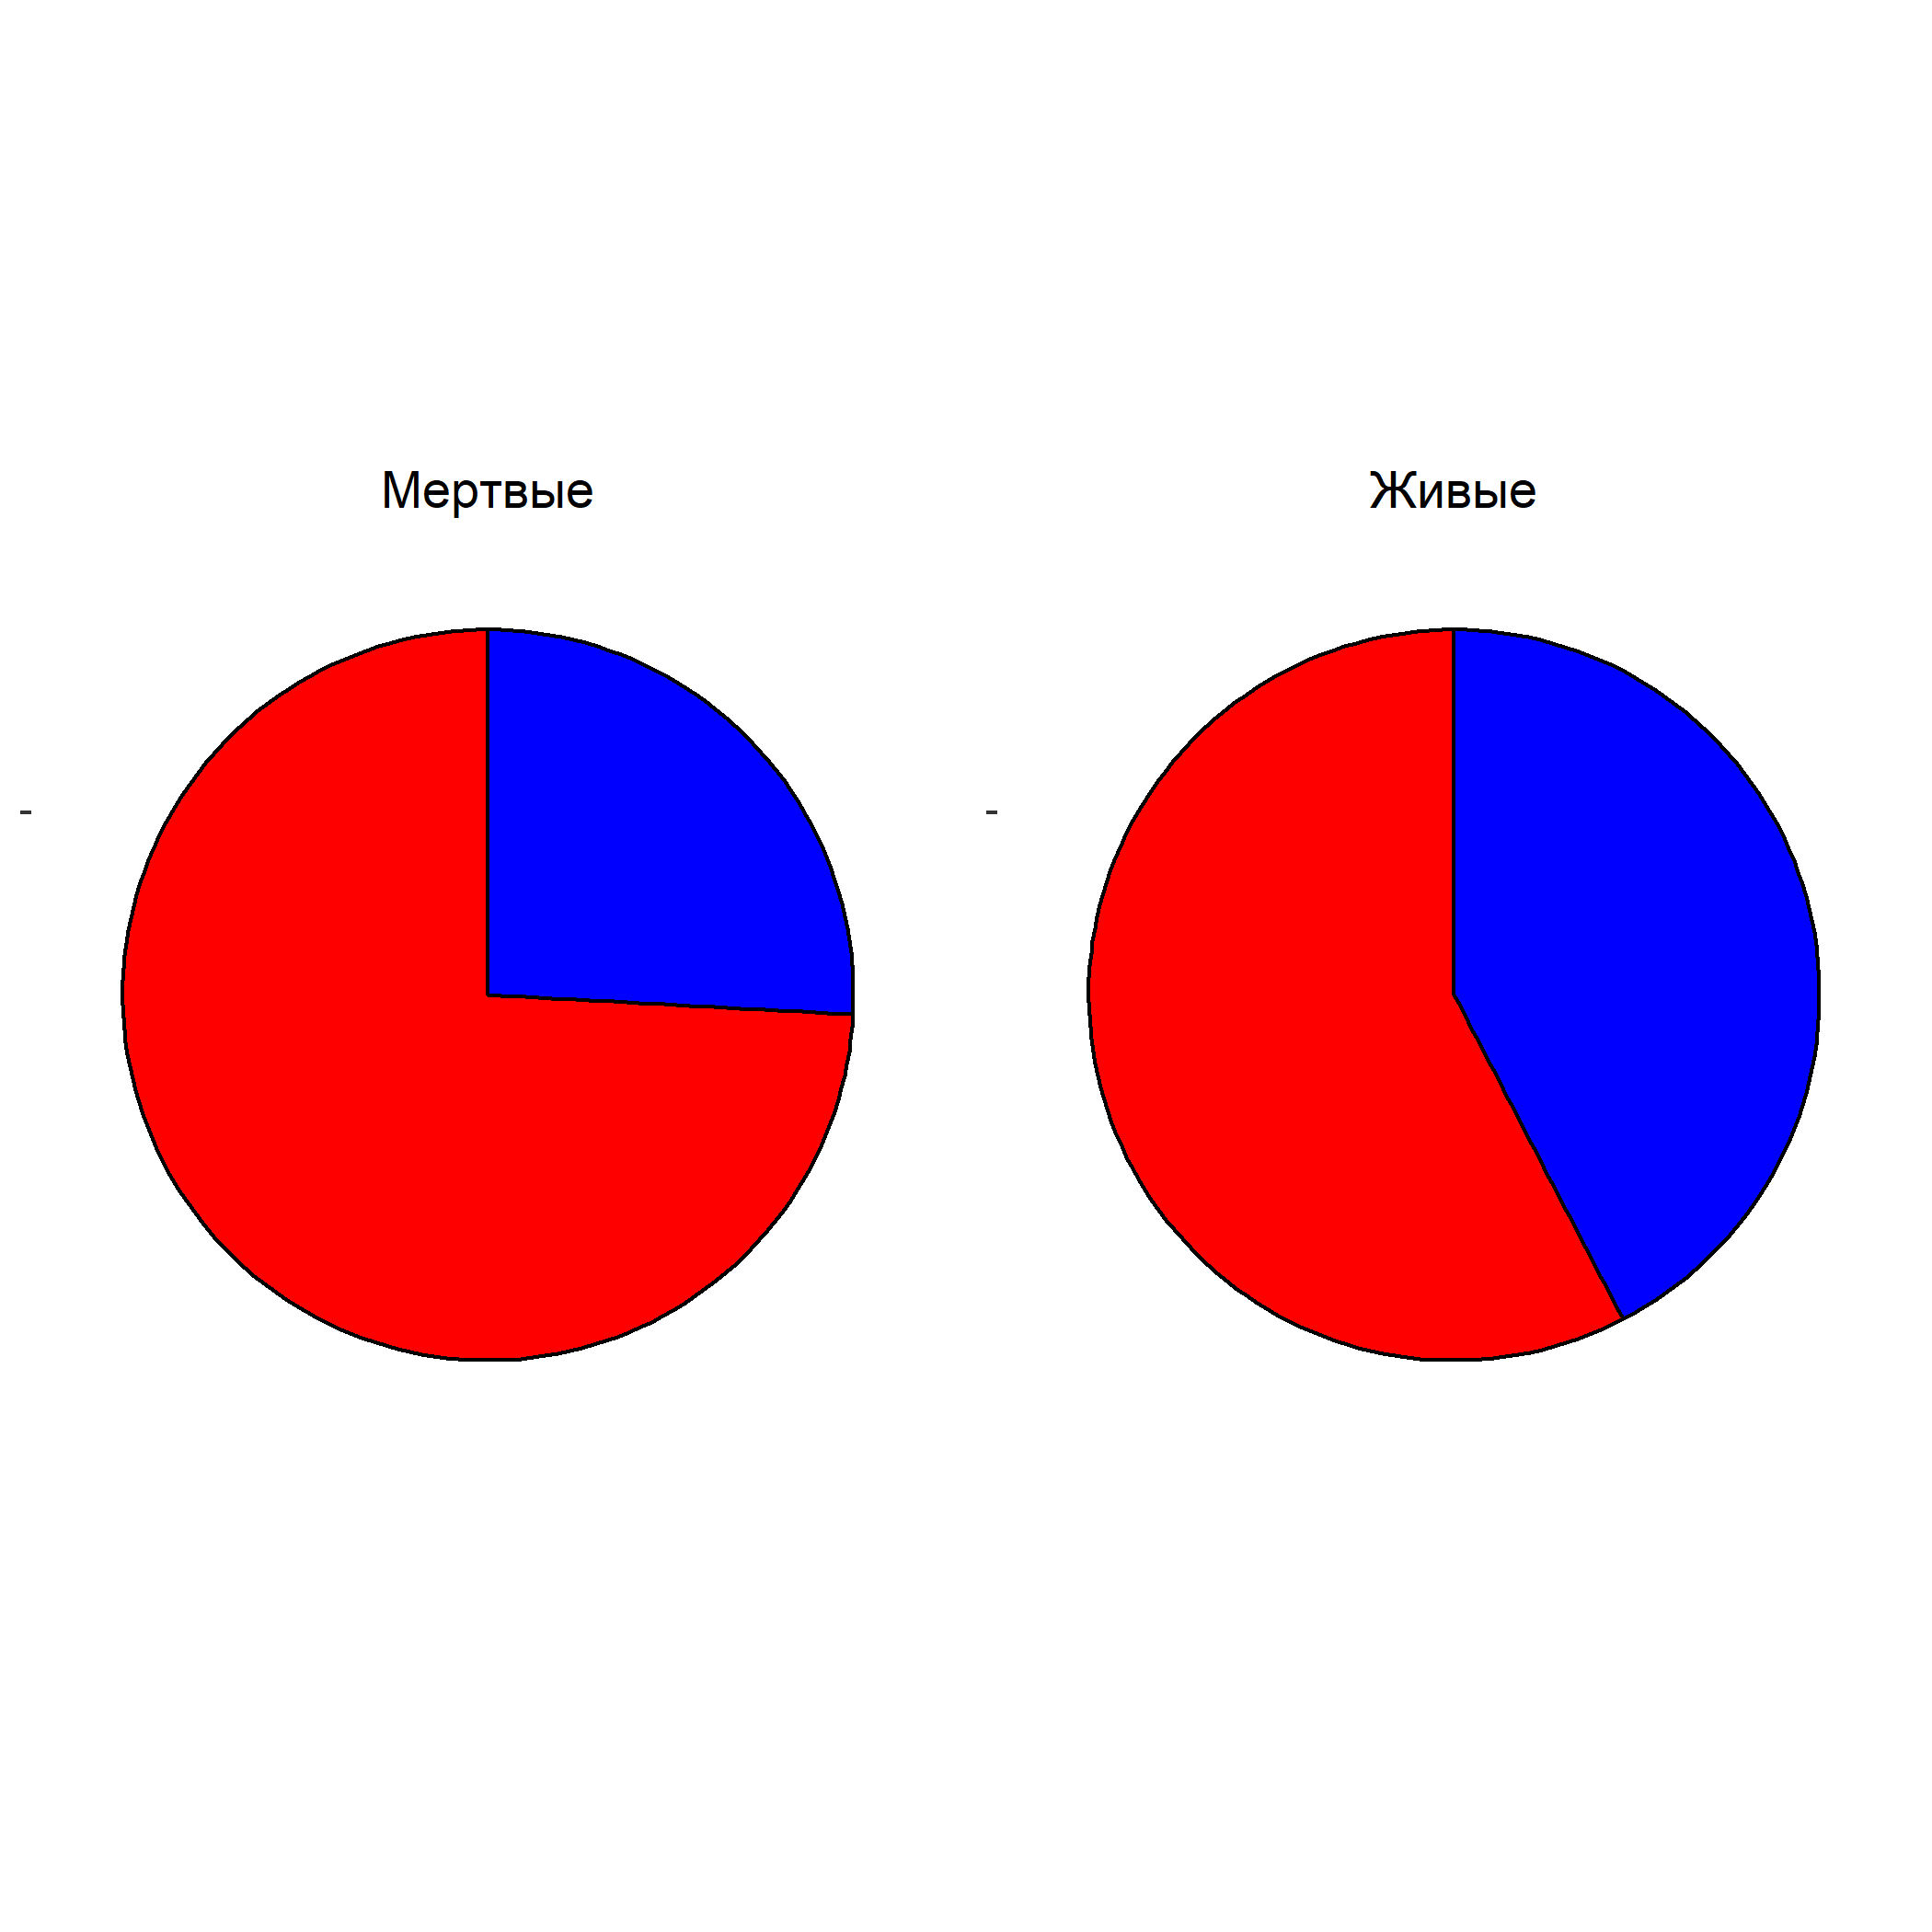
\includegraphics[width=0.9\linewidth]{Pay_charts_hem.png}
			\captionof{figure}{\color{Green} Соотношение численностей Т- (красный сектор) и Е-морфотипов (синий сектор) среди живых и съеденных моллюсков в местах питания куликов-сорок.}
			\label{Pay_charts_hem}
		\end{center}
\end{minipage}\hspace{1cm}
%
\begin{minipage}[t]{0.46\linewidth}		
	\begin{center}\vspace{0.1cm}
			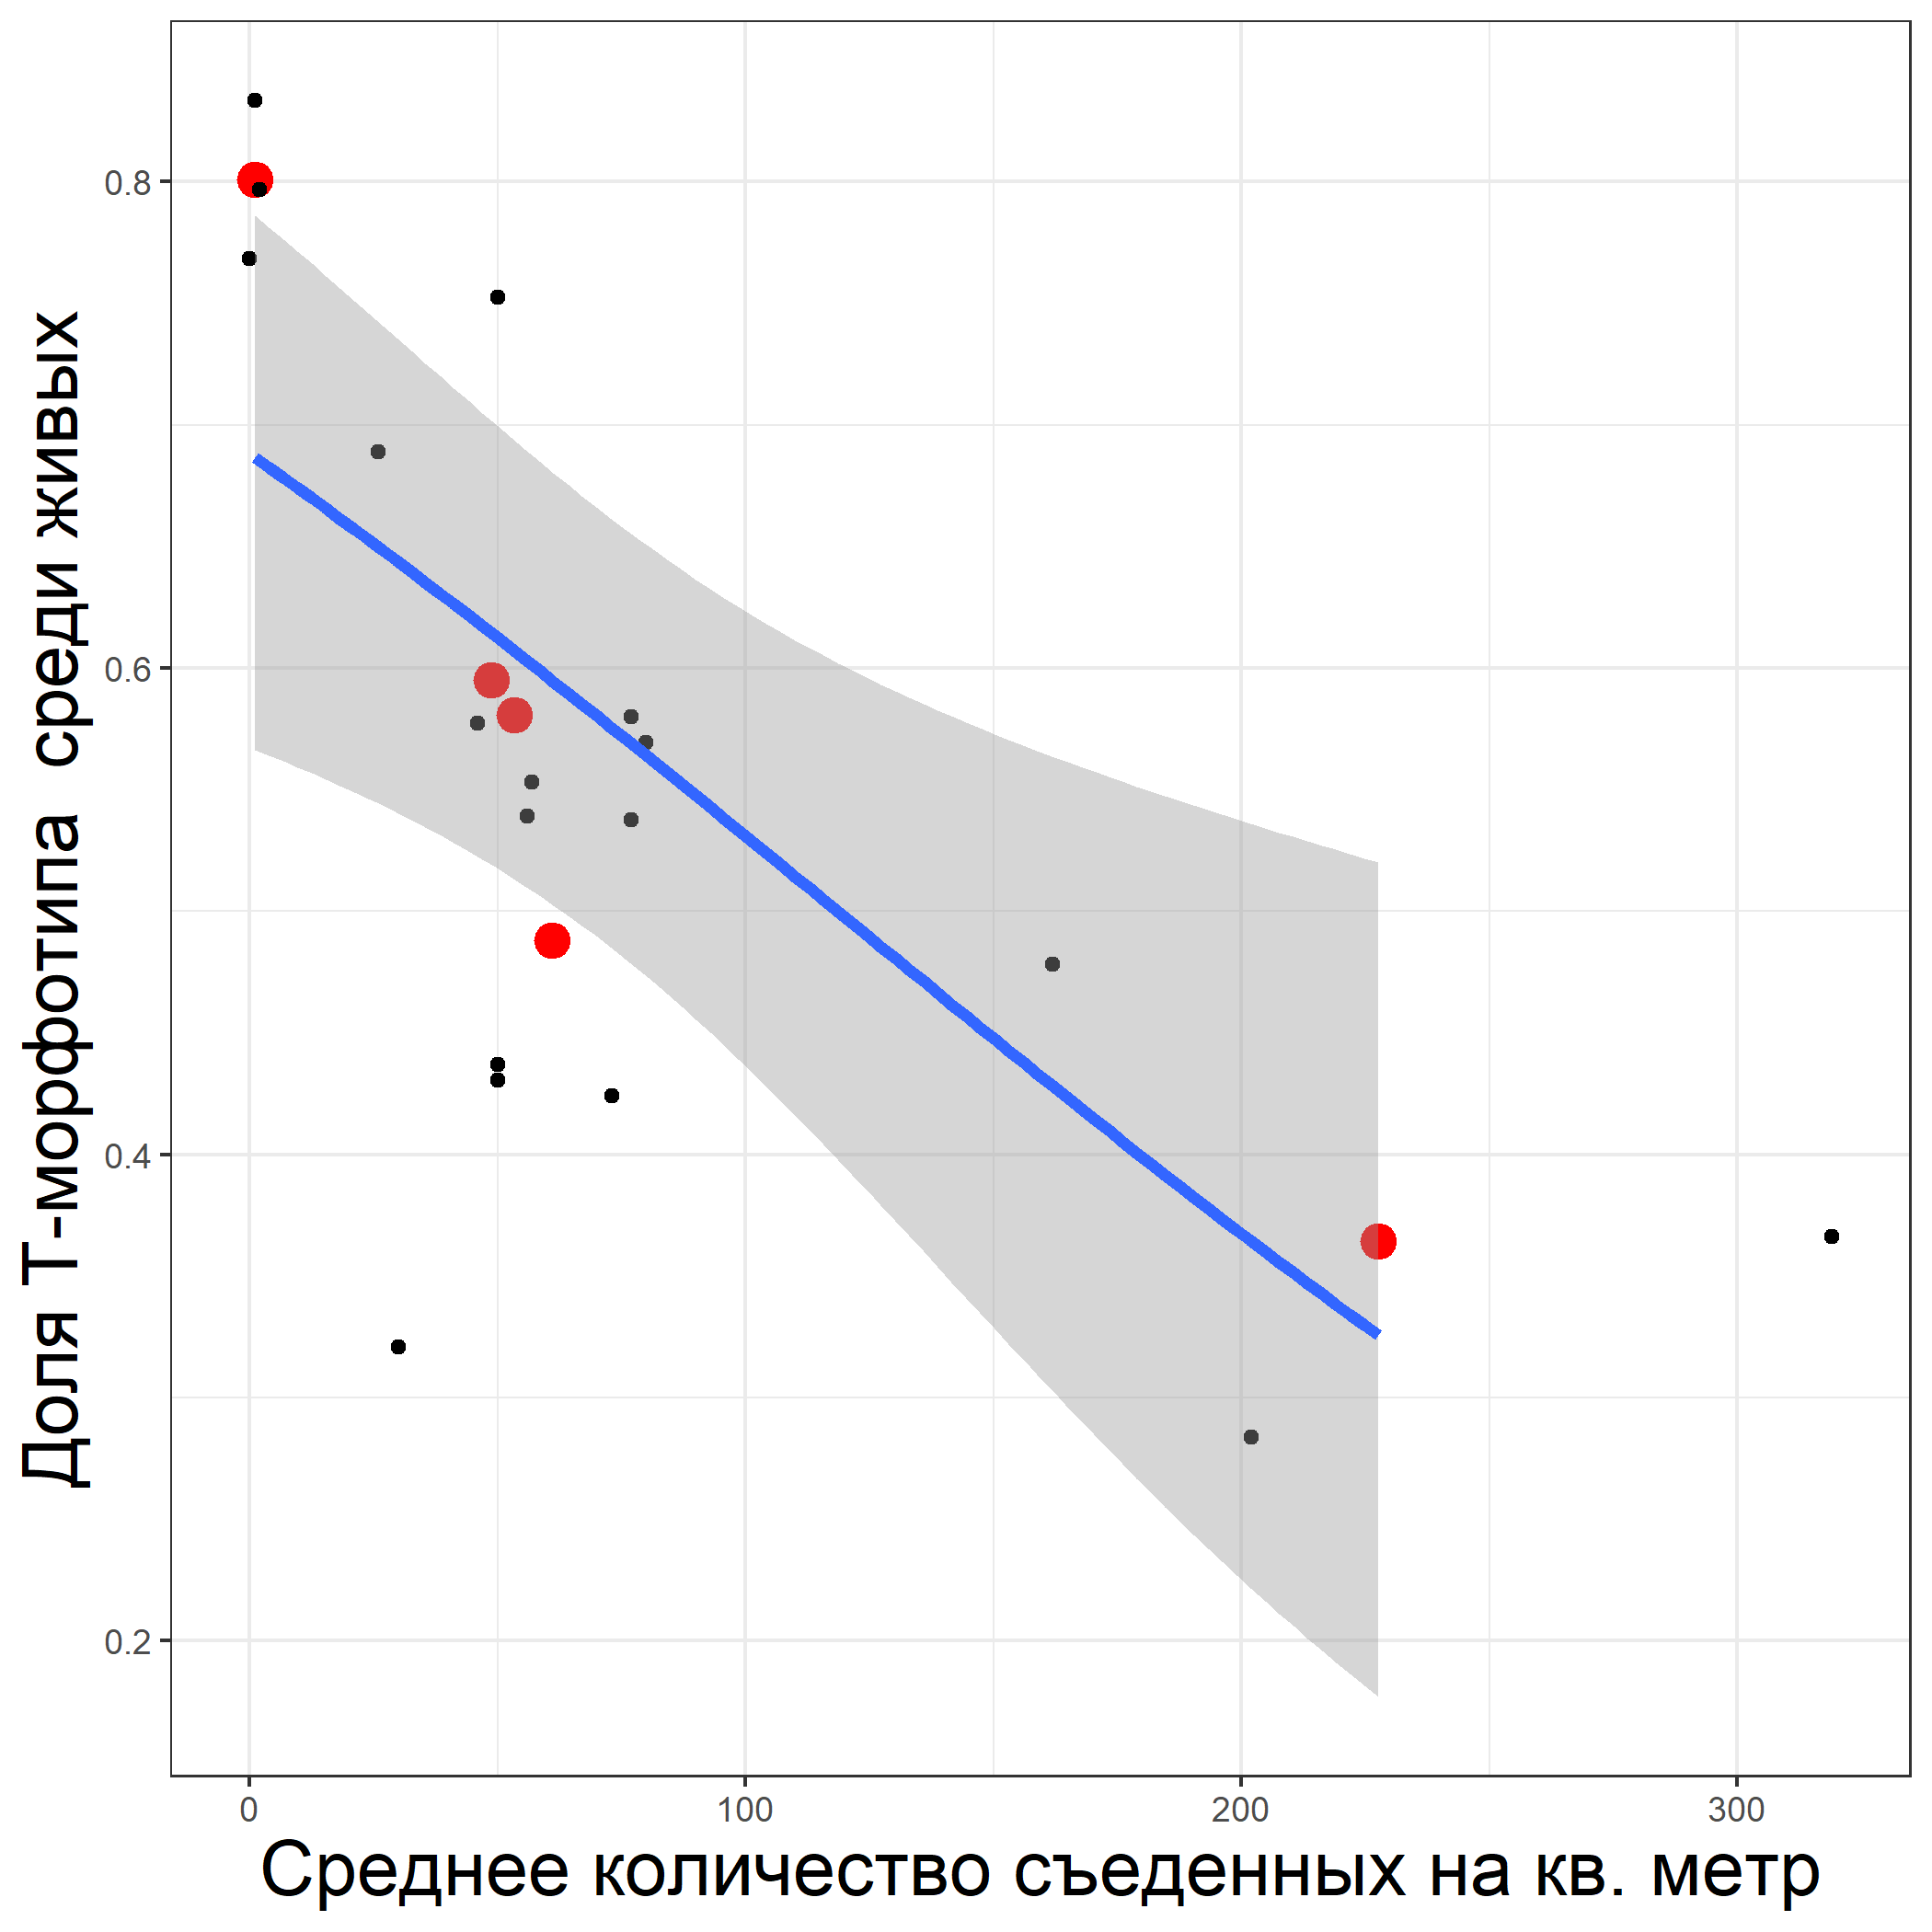
\includegraphics[width=0.9\linewidth]{N_dead_Prop_T_hem.png}
			\captionof{figure}{\color{Green} Зависимость доли мидий Т-морфотипа среди живых мидий от обилия съеденных моллюсков (степени воздействия куликов-сорок).}
			\label{N_dead_Prop_T_hem}
		\end{center}
\end{minipage}\vspace{0.5cm}



Кулики-сороки предпочитают более крупых мидий (рис. \ref{Fig_siz_hem}.

Обилие живых моллюсков (рис. \ref{Baster_Ndead}) падает по мере увеличения обилия створок съеденных мидий.Интенсивное питание куликов может заметно сокращать обилие жертв. По количеству створок погибших моллюсков можно судить о степени воздействия хищника.

Доля Т-морфотипа среди съеденных моллюсков (рис.  \ref{Pay_charts_hem}) выше, чем доля таких мидий среди живых особей. Кулки предпочитают атаковать мидий Т-морфотипа. 
На фоне увеличения доли съеденных мидий наблюдалось падение относительного обилия мидий Т-морфотипа среди живых особей (рис. \ref{N_dead_Prop_T_hem}).

\end{minipage}





%
% 		%----------------------------------------------------------------------------------------
% 		%	CONCLUSIONS
% 		%----------------------------------------------------------------------------------------
%
% 		\color{SaddleBrown} % SaddleBrown color for the conclusions to make them stand out
%
% 		\section*{Заключение}
%
% 		\begin{itemize}
% 			\item Оба вида хищников могут эффективно сокращать частоту M.trossulus в смешанных поселениях.
% 			\item Концентрация M.trossulus в куту Канадалкшского залива может быть связана с малым обилием хищников в этом районе.
% 		\end{itemize}
%
% 		\color{DarkSlateGray} % Set the color back to DarkSlateGray for the rest of the content

		%----------------------------------------------------------------------------------------
		%	FORTHCOMING RESEARCH
		%----------------------------------------------------------------------------------------
		
		% \section*{Forthcoming Research}
		% 
		% Vivamus molestie, risus tempor vehicula mattis, libero arcu volutpat purus, sed blandit sem nibh eget turpis. Maecenas rutrum dui blandit lorem vulputate gravida. Praesent venenatis mi vel lorem tempor at varius diam sagittis. Nam eu leo id turpis interdum luctus a sed augue. Nam tellus.
		% 
		%----------------------------------------------------------------------------------------
		%	REFERENCES
		%----------------------------------------------------------------------------------------
		% 
		% \nocite{*} % Print all references regardless of whether they were cited in the poster or not
		% \bibliographystyle{abbrvnat} % Plain referencing style
		% \bibliography{My_bibliograhy} % Use the example bibliography file sample.bib
		% 
		%----------------------------------------------------------------------------------------
		%	ACKNOWLEDGEMENTS
		%----------------------------------------------------------------------------------------
		
		% \section*{Acknowledgements}
		% 
		% Etiam fermentum, arcu ut gravida fringilla, dolor arcu laoreet justo, ut imperdiet urna arcu a arcu. Donec nec ante a dui tempus consectetur. Cras nisi turpis, dapibus sit amet mattis sed, laoreet.
		% 
		%----------------------------------------------------------------------------------------
		
		
% \end{multicols}
	
\end{document}
